\documentclass{article}


\usepackage[T1]{fontenc}
\usepackage[utf8]{inputenc}
\usepackage[french,german,english]{babel}

\usepackage{fullpage}
\usepackage{graphicx,xcolor}
\usepackage{url}
\usepackage{amsmath}

\usepackage{subfigure}


\begin{document}

\begin{titlepage}
\begin{center}
%\large
\sffamily


\null\vspace{2cm}
{\huge PCL Toyota Code Sprint 2.0 - Superquadrics} \\[24pt]
\textcolor{gray}{{\\ Alexandru - Eugen Ichim}}
    
\vfill

\begin{tabular} {cc}
\hspace{1cm}
\parbox{0.4\textwidth}{
\includegraphics[width=6cm]{figures/logos}}
\hspace{4cm}
&
\parbox{0.7\textwidth}{%
	Open Perception Inc. \\ \\ \\
%
\small
Supervised by:\\[4pt]
%
    Dr. Joseph Djugash\\
    Dr. Radu B. Rusu\\[12pt]
%
2013}
\end{tabular}
\end{center}
\vspace{2cm}
\end{titlepage}


%%%%%%%%%%%%%%%%%%%%%%%%%%%%%%%%%%%%%%%%%%%%%%%%%%%%%%%%%%%%
%%%%%%%%%%%%%%%%%%%%%%%%%%%%%%%%%%%%%%%%%%%%%%%%%%%%%%%%%%%%

\tableofcontents
\newpage

\section {Introduction}

\subsection {Code Sprint}
A code sprint is an accelerated research and development program, inspired by the Google Summer of Code model, and organised within the Point Cloud Library project by the host foundation, Open Perception Inc. PCL developers are paired with senior researchers and engineers from various institutions for extended R\&D work with financial backup.

The first code sprint in which Toyota got involved was done in 2012, and one of the projects was that of implementing novel smoothing algorithms \cite{tocs_final_report}.

\subsection {Target}
The target of the current code sprint is that of analysing the possibilities of using superquadric object representation in robotics-oriented computer vision tasks such as object detection. 

The structure of this report is as follows. In this section we continue by introducing the concept of superquadrics and some mathematical background, as well as sources of datasets we have used for development. Next, in Section \ref{sec:sampling}, we look into techniques for sampling the superquadric equation in order to get point clouds and meshes. Section \ref{sec:fitting} shows the approaches we implemented for fitting superquadric objects into point clouds, with the extension of fully describing a point set as a collection of non-overlapping superquadrics. We then look into how to efficiently find objects for which we now the parametric representation in a new point cloud - Section \ref{sec:detection}. Finally, we show a complete demo using an RGB-D sensor in Section \ref{sec:tabletop_demo} and finalise with concluding remarks in Section \ref{sec:conclusion}.


\subsection {Superquadrics}

\subsubsection*{History}
The concept of superquadrics was first introduced in the Computer Graphics community in \cite{1673799}, as a means of versatile parametric object modelling. The mathematical details have been extended in the work of Jakli\v{c} et al. \cite{SQ_2000}. Just like quadrics, superquadrics can be split into superellipsoids, superhyperboloids of one piece, superhyperboloids of two pieces and supertoroids, but for the purpose of our work, we only focused on superellipsoids (see Figure \ref{fig:superquadric_family}).

\begin{figure}
\centering
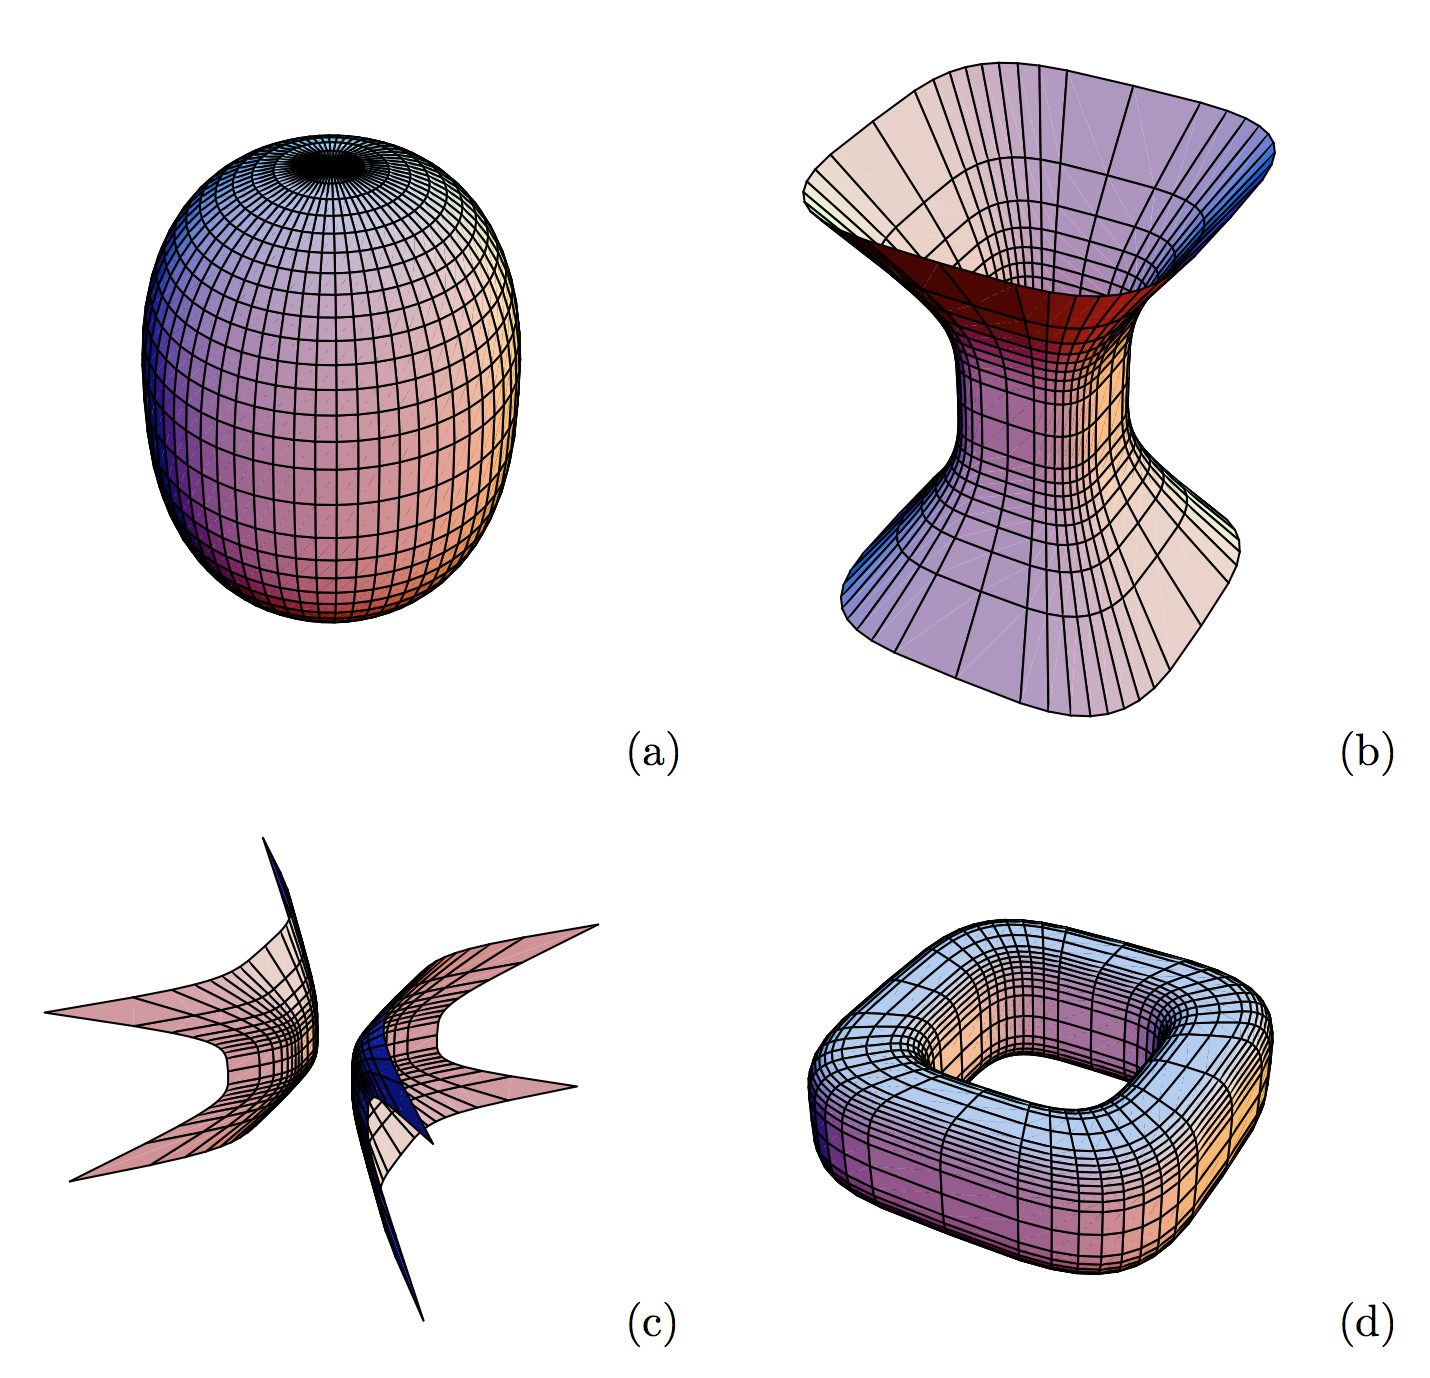
\includegraphics[width=0.5\columnwidth]{figures/superquadric_family}
\caption{Family of superquadrics: (a) superellipsoid, (b) superhyperboloid of one sheet, (c) superhyperboloid of two sheets, (d) supertoroid}
\label{fig:superquadric_family}
\end{figure}

\subsubsection*{Mathematical Definition}
\label{sec:math}
They are created from two two-dimensional curves (a horizontal and a vertical curve) that form a three-dimensional surface under spherical product. For example, a unit sphere is created as the spherical product of a half circle in the plane orthogonal to $(x, y)$ crossed with the full circle in the $(x, y)$ plane.

\begin{equation}
m (\eta) = \begin{pmatrix} \cos {\eta} \\ \sin{\eta} \end{pmatrix} \textnormal{, with: } \eta \in [-\pi/2, \pi/2] 
\end{equation}

\begin{equation}
h(\omega) = \begin{pmatrix} \cos {\omega} \\ \sin {\omega} \end{pmatrix} \textnormal{, with: } \omega \in [-\pi, \pi)
\end{equation}

The sphere becomes:

\begin{equation}
r (\eta, \omega) = m (\eta) \oplus h (\omega) = \begin{pmatrix} \cos{\eta} \cos{\omega} \\ \cos{\eta} \sin{\omega} \\ \sin{\omega} \end{pmatrix}
\end{equation}

A superellipsoid can be obtained by the spherical product of two superellipses of the form:

\begin{equation}
\left(\frac{x}{a}\right)^{\frac{2}{\epsilon}} + \left(\frac{y}{b}\right)^{\frac{2}{\epsilon}} = 1
\end{equation}

\begin{equation}
s(\theta) = \begin{pmatrix} a \cos^\epsilon{\theta} \\ b \sin^\epsilon {\theta} \end{pmatrix} \textnormal{, with } \theta \in [-\pi, \pi]
\end{equation}

\begin{equation}
r (\eta, \omega) = s_1 (\eta) \oplus s_2 (\omega) = \begin{pmatrix} \cos^{\epsilon_1} {\eta} \\ a_3 \sin^{\epsilon_1} {\eta} \end{pmatrix} \oplus \begin{pmatrix} a_1 \cos^{\epsilon_2} {\omega} \\ a_2 \sin^{\epsilon_2} {\omega} \end{pmatrix} = \begin{pmatrix} a_1 \cos^{\epsilon_1} {\eta} \cos^{\epsilon_2} {\omega} \\ a_2 \cos^{\epsilon_1} {\eta} \sin^{\epsilon_2} {\omega} \\ a_3 \sin^{\epsilon_1}{\eta}\end{pmatrix} \textnormal{, with } \eta \in [-\pi/2, \pi/2], \omega \in [-\pi, \pi)
\end{equation}

The five parameters of a superellipsoid are as follows:

\begin{itemize}
	\item {\textbf{$a_1$, $a_2$, $a_3$} - scaling factors along the three axes}
	\item {\textbf{$\epsilon_1$} - the shape of the superellipsoid cross section in a plane orthogonal to the $(x, y)$ plane and containing the $z$-axis}
	\item {\textbf{$\epsilon_2$} - the shape of the superellipsoid cross section parallel to the $(x, y)$ plane}	
\end{itemize}

% TODO Generate superellipsoids with various parameters: vary a,b,c, bigger e1, bigger e2 - 7 figures in total

The implicit equation of a superellipsoid is thus:

\begin{equation}
\left(\left(\frac{x}{a_1}\right)^{\frac{2}{\epsilon_2}} + \left(\frac{y}{a_2}\right)^{\frac{2}{\epsilon_2}}\right)^{\frac{\epsilon_2}{\epsilon_1}} + \left(\frac{z}{a_3}\right)^{\frac{2}{\epsilon_1}} =1
\end{equation}

Because of the inside-outside functions that describe superquadrics, they can be easily manipulated by means of solid boolean operations such as union, intersection and subtraction.

\subsubsection*{Numerical Issues}
There are some issues we need to take into consideration when writing code that involves the usage of superquadrics. All the powers in the implicit function are of the form $2p$: $2/\epsilon_1$, $2/\epsilon_2$, and we compute them in the order $x^{(2p)}=(x^2)^p$ so that they are always positive. In the case of the explicit function, all the powers are actually signed power functions, and are treated as follows:

\begin{equation}
x^p = sgn(x) |x|^p = \left\{
	\begin{array}{ll}
		|x|^p  & \textnormal{if } x \geq 0 \\
		-|x|^p & \textnormal{if } x < 0
	\end{array}
\right.
\end{equation}


Because of the limitation of the range of real numbers a 64-bit system can compute within, we need to clamp the $\epsilon_1$ and $\epsilon_2$ parameters in the interval $(0.1, 1.9)$. Values beyond this range do not introduce a lot more expressiveness to the objects, but create numerical problems as $\frac{\epsilon_2}{\epsilon_1}$ becomes very large.

\subsection {Datasets}
For the purpose of this work, we gathered data from multiple sources:

\begin{itemize}
	\item{\textbf{Created manually} - using Google Sketchup - Figure \ref {fig:sketchup}}
	\item{\textbf{Trimble 3D Warehouse} - \url{http://sketchup.google.com/3dwarehouse/} - Figure \ref {fig:trimble_warehouse}}
	\item{\textbf{Scanned with an RGB-D camera} - multiple frames registered with PCL KinFu - Figure \ref{fig:kinfu_datasets}}
\end{itemize}

\begin{figure}
\centering
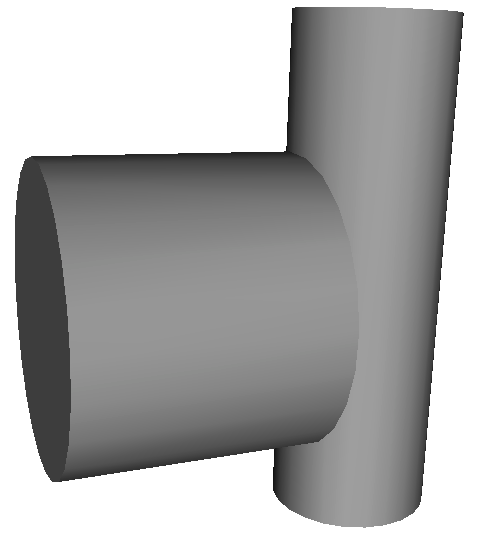
\includegraphics[width=0.2\columnwidth]{figures/2_components}
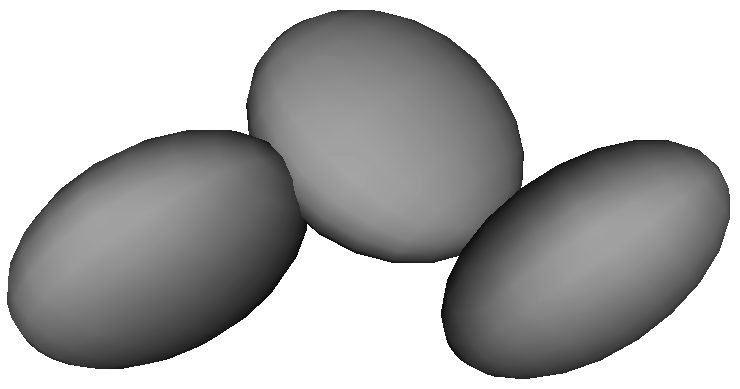
\includegraphics[width=0.3\columnwidth]{figures/3_components}
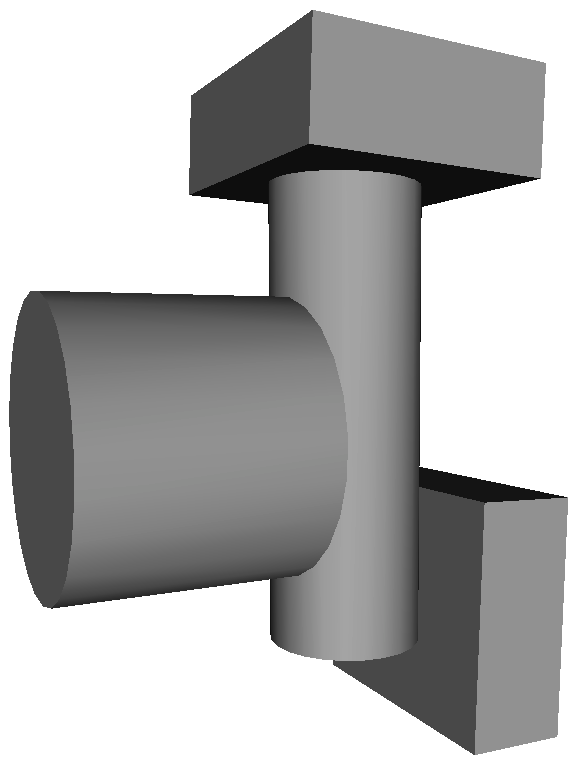
\includegraphics[width=0.2\columnwidth]{figures/4_components}
\caption {Example datasets created with Google Sketchup.}
\label{fig:sketchup}
\end{figure}

\begin{figure}
\centering
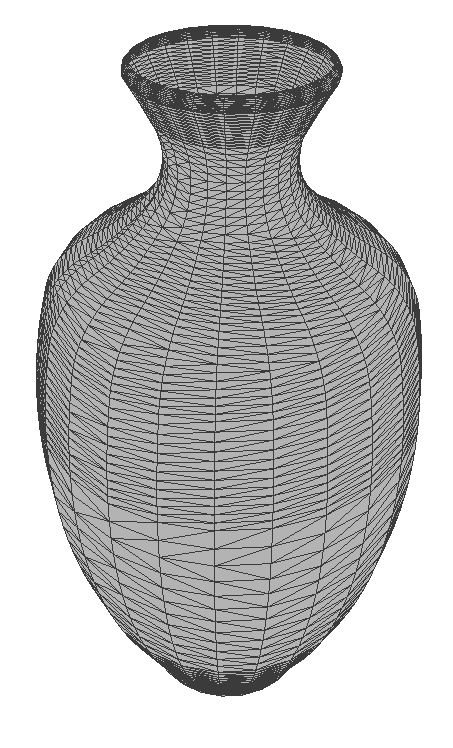
\includegraphics[width=0.2\columnwidth]{figures/vase_1}
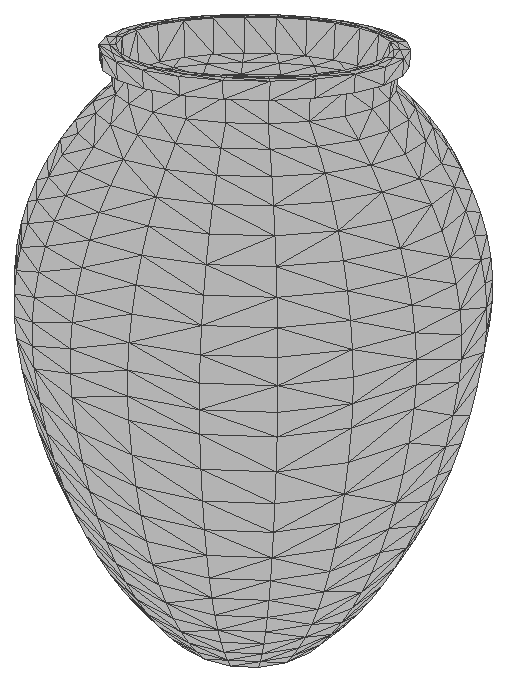
\includegraphics[width=0.2\columnwidth]{figures/vase_2}
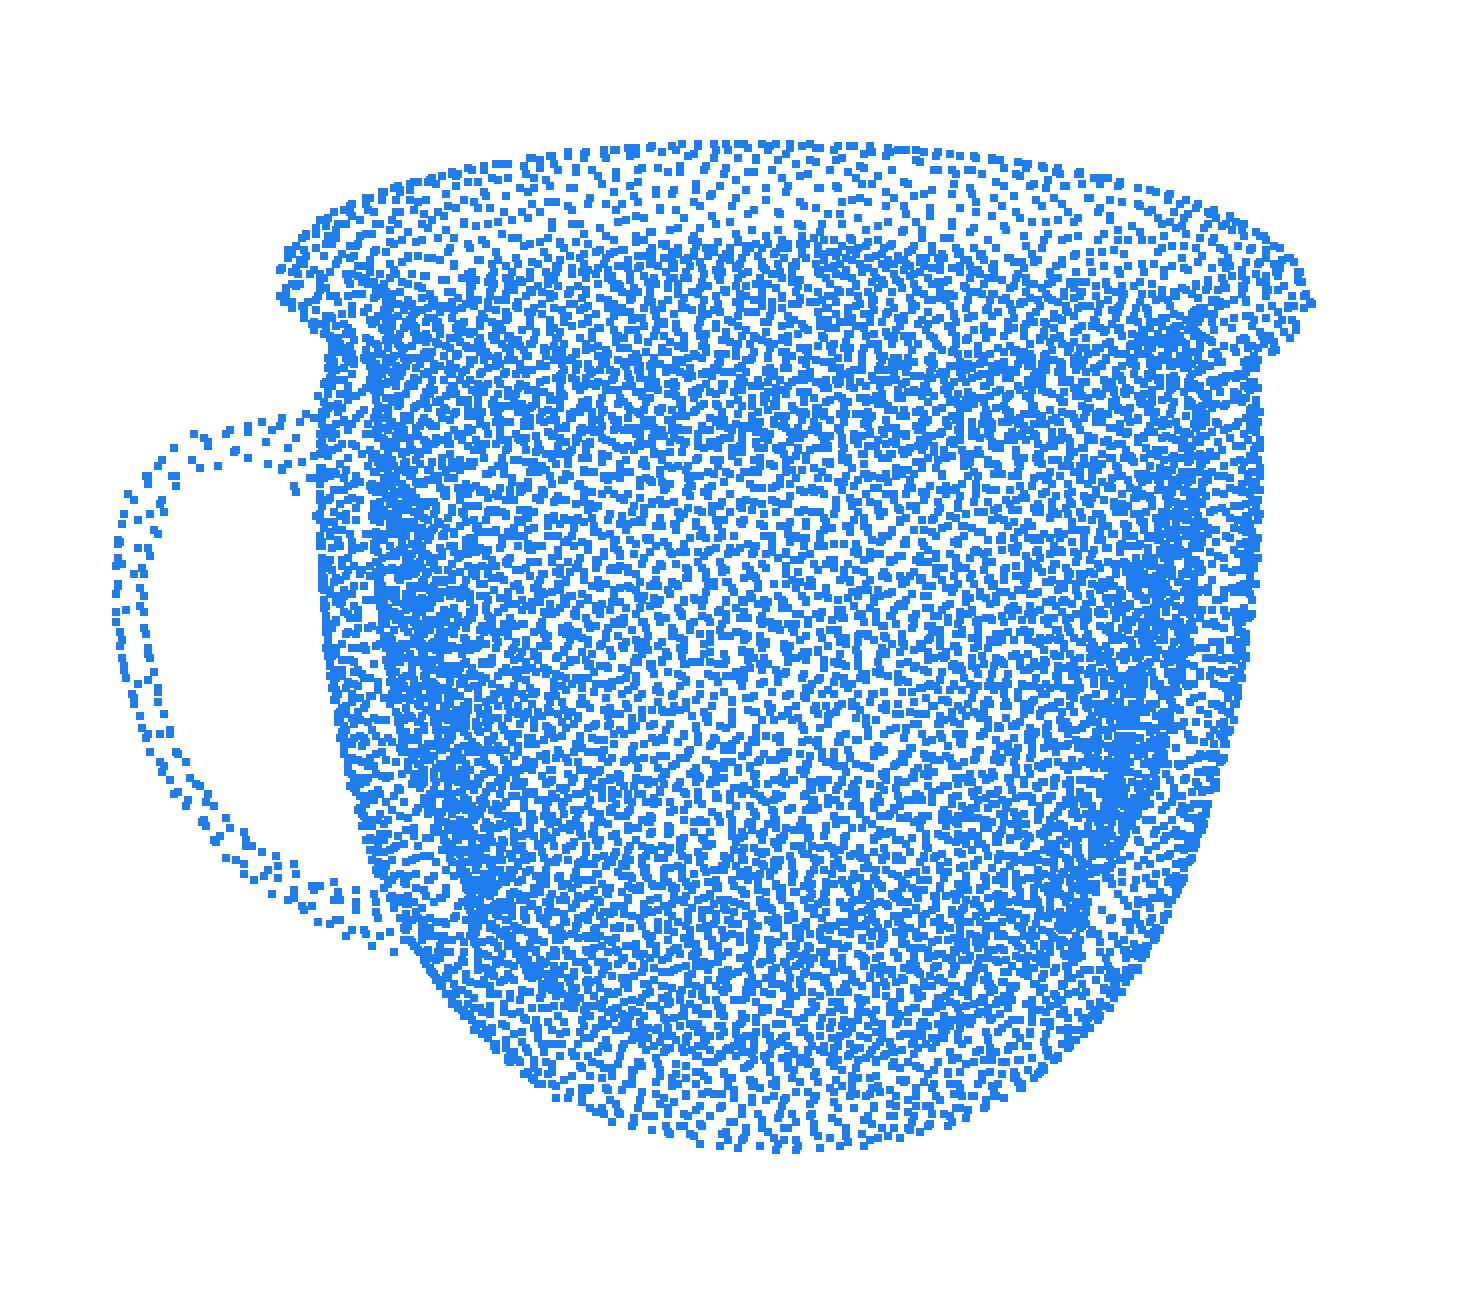
\includegraphics[width=0.3\columnwidth]{figures/cup}
\caption {Example datasets downloaded from the Trimble 3D Warehouse.}
\label{fig:trimble_warehouse}
\end{figure}
		
\begin{figure}
\centering

\includegraphics[width=0.3\columnwidth]{figures/kinfu_1}
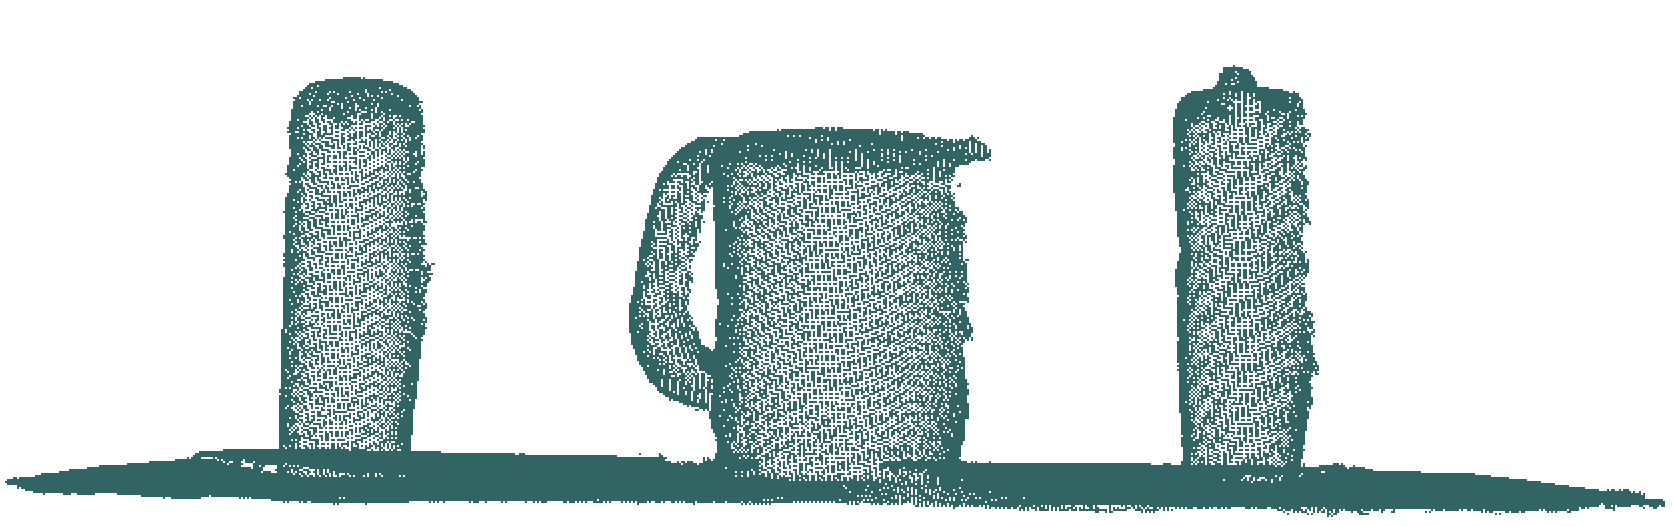
\includegraphics[width=0.3\columnwidth]{figures/kinfu_2}
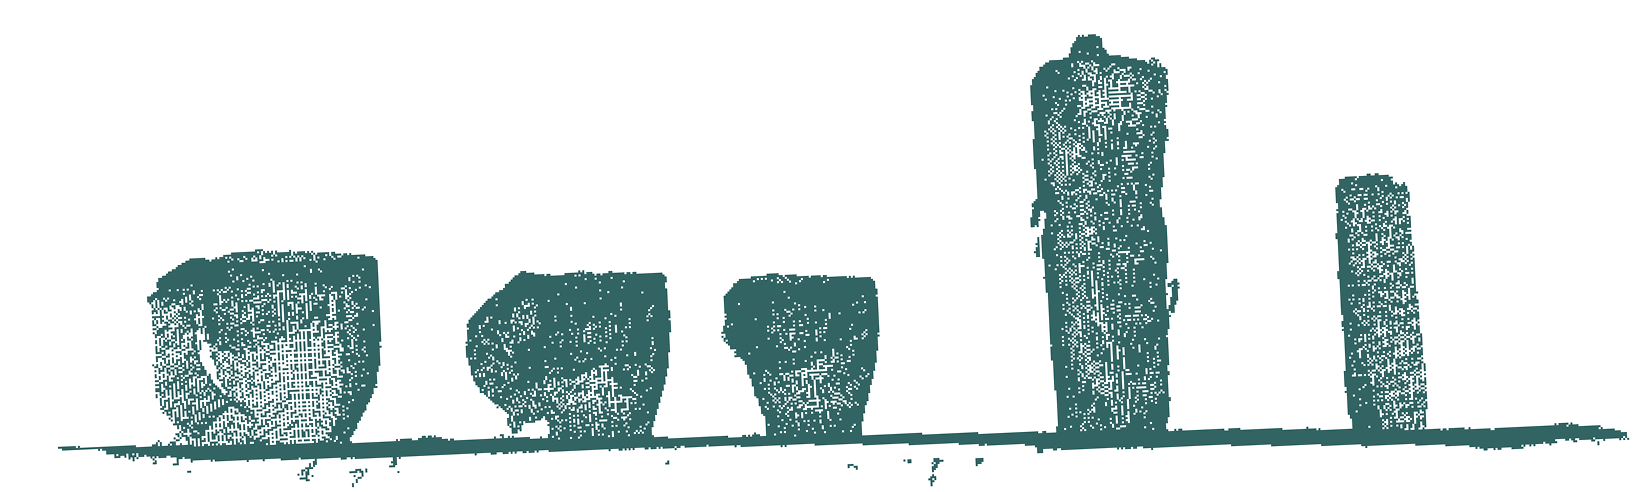
\includegraphics[width=0.3\columnwidth]{figures/kinfu_3}
\caption {Example datasets created using PCL KinFu.}
\label{fig:kinfu_datasets}
\end{figure}
		
		
		
	


%%%%%%%%%%%%%%%%%%%%%%%%%%%%%%%%%%%%%%%%%%%%%%%%%%%%%%%%%%%%
%%%%%%%%%%%%%%%%%%%%%%%%%%%%%%%%%%%%%%%%%%%%%%%%%%%%%%%%%%%%
\section {Sampling}
\label{sec:sampling}

Sampling superquadrics is important as it allows for easy visualization and for evaluating fitting or registration errors. We have tried multiple ways of doing this, as will be explained in this section.

\subsection {VTK}

Using the Visualization ToolKit library, the code for generating a superquadric centered at the origin is simply:

\begin{verbatim}
    vtkSmartPointer<vtkSuperquadricSource> superquadricSource = 
       vtkSmartPointer<vtkSuperquadricSource>::New();
    superquadricSource->SetPhiRoundness (epsilon_1);
    superquadricSource->SetThetaRoundness (epsilon_2);
    superquadricSource->SetScale (a, b, c);
    superquadricSource->SetPhiResolution (1000);
    superquadricSource->SetThetaResolution (1000);
    superquadricSource->SetSize (1.);
\end{verbatim}

As the code suggests (setting $\phi$ and $\theta$ resolutions), this does nothing but uniformly sample the parameter space for the two angles and generate points using the explicit equation. This source can be then connected to a renderer and used to display the generated mesh - see Figure \ref{fig:sampling_VTK}.

\begin{figure}
\centering
\includegraphics[width=0.25\columnwidth]{figures/sampling_VTK_solid}
\hspace {1cm}
\includegraphics[width=0.25\columnwidth]{figures/sampling_VTK_wireframe}
\caption {Superquadric sampling using the VTK library.}
\label{fig:sampling_VTK}
\end{figure}


\subsection {Explicit}

Here, we uniformly sample the two angular parameters of the superquadric, and set the correct mesh connectivity. As with the VTK results, we see that the meshes are not spatially sampled in an uniform way - there are not enough points around the corners and the middle of the shape - see Figure \ref{fig:sampling_explicit}.

\begin{figure}
\centering
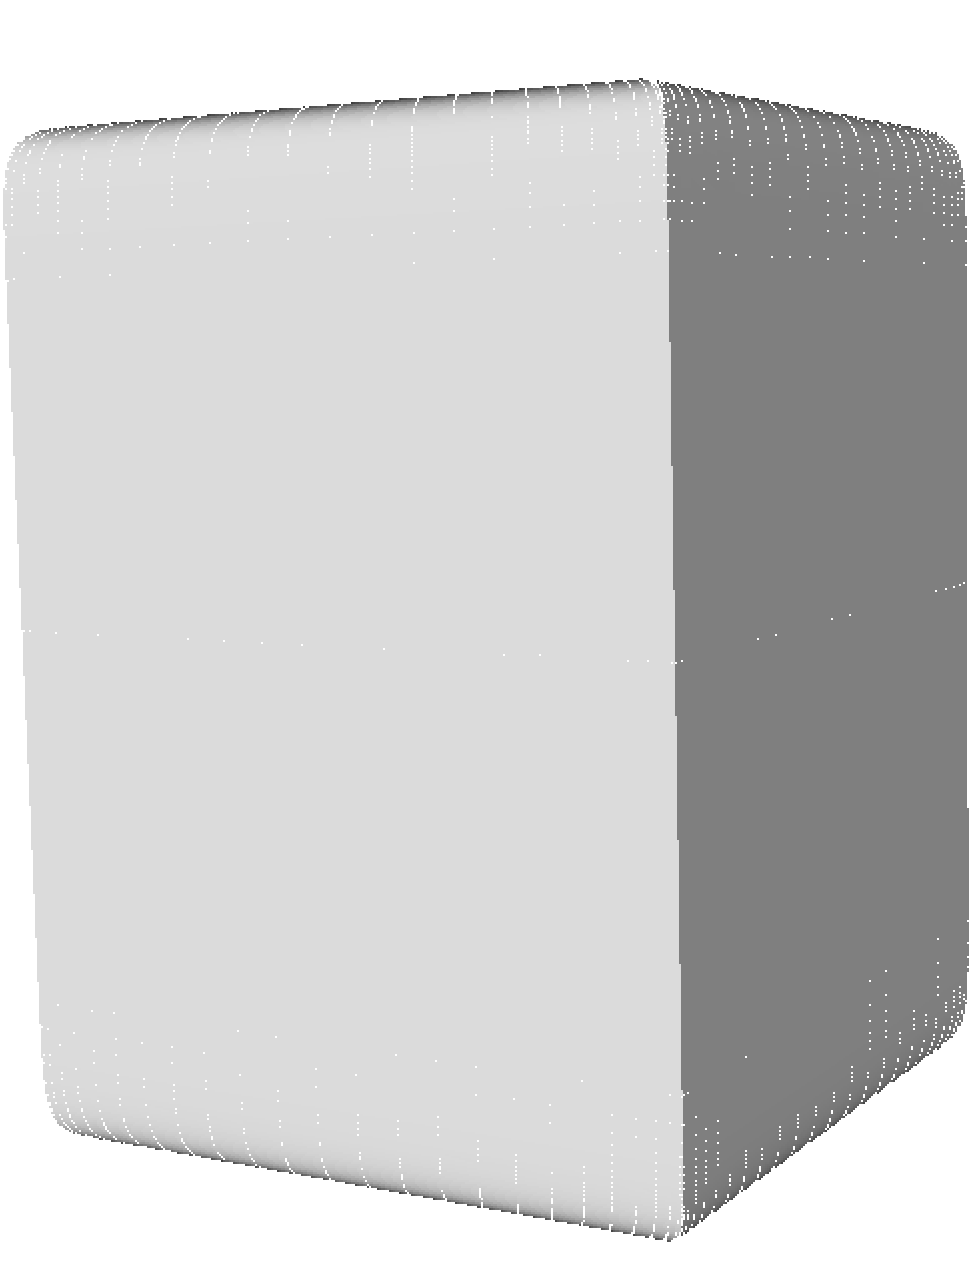
\includegraphics[width=0.25\columnwidth]{figures/sampling_explicit_solid}
\hspace {1cm}
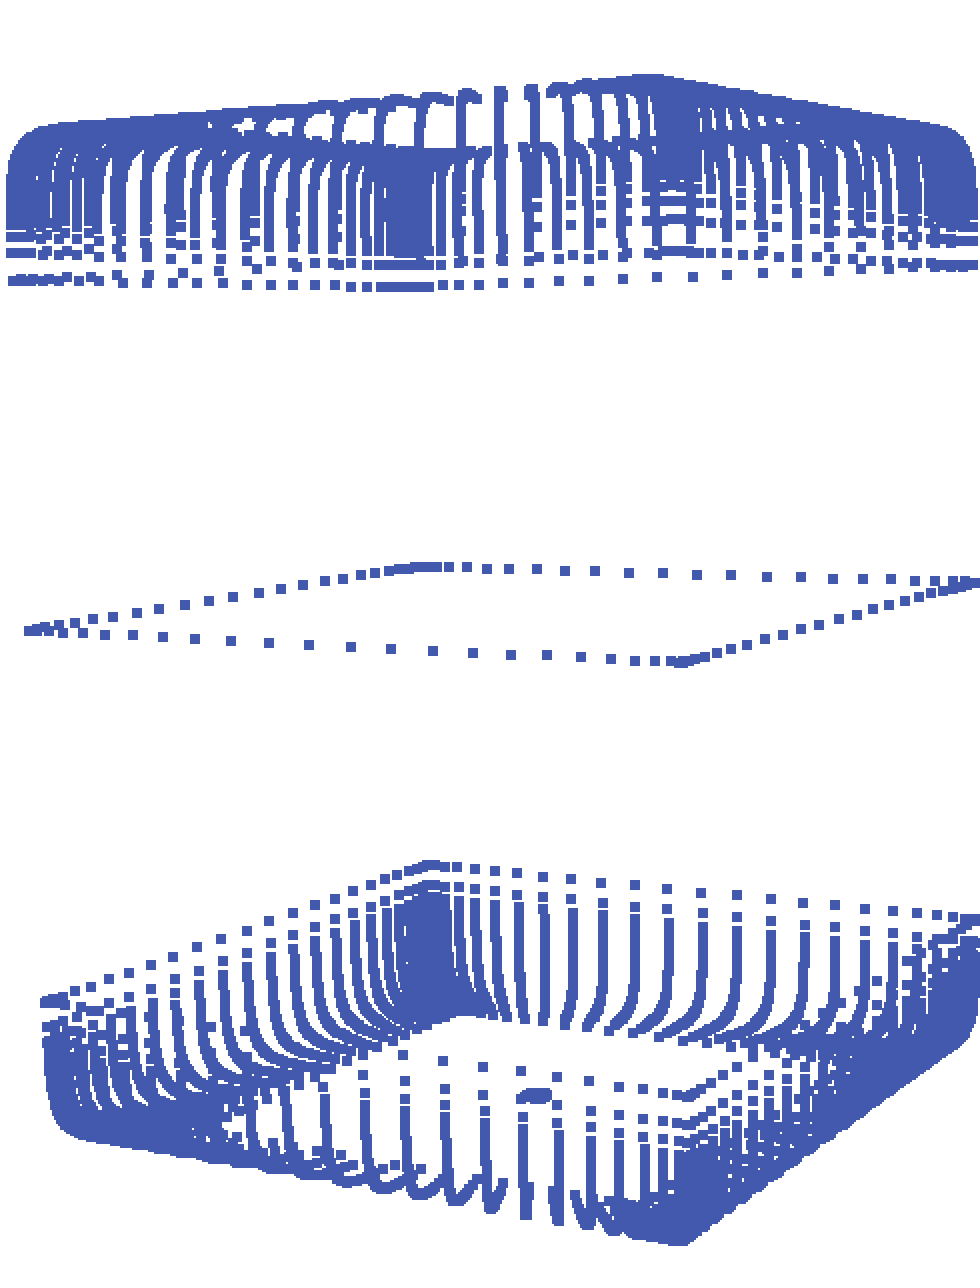
\includegraphics[width=0.25\columnwidth]{figures/sampling_explicit_cloud}
\caption {Superquadric sampling by uniformly sampling the angular parameter space.}
\label{fig:sampling_explicit}
\end{figure}


\subsection {Uniform Spatial Sampling}

In order to obtain uniform spatial sampling, which is much more suitable for computing errors, we need to look deeper into the problem. \cite{Pilu95equal-distancesampling} suggests a fast and mathematically sound solution. We start our derivation with the implicit and explicit equations of a superellipse:

\begin{equation}
\left(\frac{x}{a_1}\right)^{2/\epsilon} + \left(\frac{y}{a_2}\right)^{2/\epsilon} = 1
\end{equation}

\begin{equation}
x(\theta) = \begin{pmatrix} a_1 \cos(\theta)^\epsilon \\ a_2 \sin(\theta)^\epsilon \end{pmatrix}
\end{equation}

The arclength between two close points $x(\theta)$ and $x (\theta + \Delta_\theta (\theta))$ on such a curve can be approximated by the euclidean distance between them:

\begin{equation}
D (\theta) = | x(\theta) - x(\theta + \Delta_\theta(\theta)) |
\end{equation}

Because $\Delta_\theta(\theta)$ is small, we can rely on a first order approximation:

\begin{equation}
D(\theta)^2 = \left( \frac{\partial}{\partial \theta} (a_1 \cos (\theta)^\epsilon) \Delta_\theta (\theta) \right)^2 + 
\left( \frac{\partial}{\partial \theta} (a_2 \sin (\theta)^\epsilon) \Delta_\theta (\theta) \right)^2
\end{equation}

which is equivalent to:

\begin{equation}
\Delta_\theta (\theta) = \frac{D(\theta)}{\epsilon} * \sqrt {\frac{ \cos (\theta) ^2 \sin (\theta) ^2} {a_1^2 \cos (\theta)^{2\epsilon} \sin(\theta)^4 + a_2^2 \sin (\theta)^{2\epsilon} \cos(\theta)^4}}
\end{equation}

By setting $D(\theta)$ to a constant spatial sampling value, the incremental updates of the angular parameter are:

\begin{eqnarray}
&& \theta_i = \theta_{i-1} + \Delta_\theta (\theta_i) \textnormal{ , with } \theta_0 = 0 \textnormal{, and } i \in \{ 1 ... N \} \textnormal {, and } \theta_N < \pi / 2 \\
&& \theta_i = \theta_{i-1} - \Delta_\theta (\theta_i) \textnormal{ , with } \theta_0 = \pi/2 \textnormal{, and } i \in \{ 1 ... N \} \textnormal {, and } \theta_N > 0
\end{eqnarray}

There are singularities at $\theta = 0$ and $\theta = \pi/2$, so we need to treat them separately. When $\theta \rightarrow 0$, the superellipse can be approximated by:

\begin{equation}
x (\theta) = \begin{pmatrix} a_1 \\ a_2 \theta ^\epsilon \end{pmatrix}
\end{equation}

resulting in:

\begin{equation}
\Delta_\theta (\theta) = \left(\frac{D (\theta)}{a_2} - \theta^\epsilon \right)^{1/\epsilon} - \theta
\end{equation}

Similarly, for $\theta \rightarrow \pi/2$:

\begin{equation}
\Delta_\theta (\theta) = \left( \frac{D(\theta)}{a_1} - (\pi/2 - \theta)^\epsilon \right)^{1/\epsilon} - (\pi/2 - \theta)
\end{equation}

The final solution is to switch between the 3 branches depending on the current value of $\theta$.

What was described until now is applied to a single superellipse. In order to spatially sample a superquadric in an uniform way, we sample one superellipse for $\epsilon_1$ and one for $\epsilon_2$ and then compute their spherical product (see Section \ref{sec:math} for details). Figure \ref{fig:sampling_smart} shows the results we obtained.

\begin{figure}
\centering
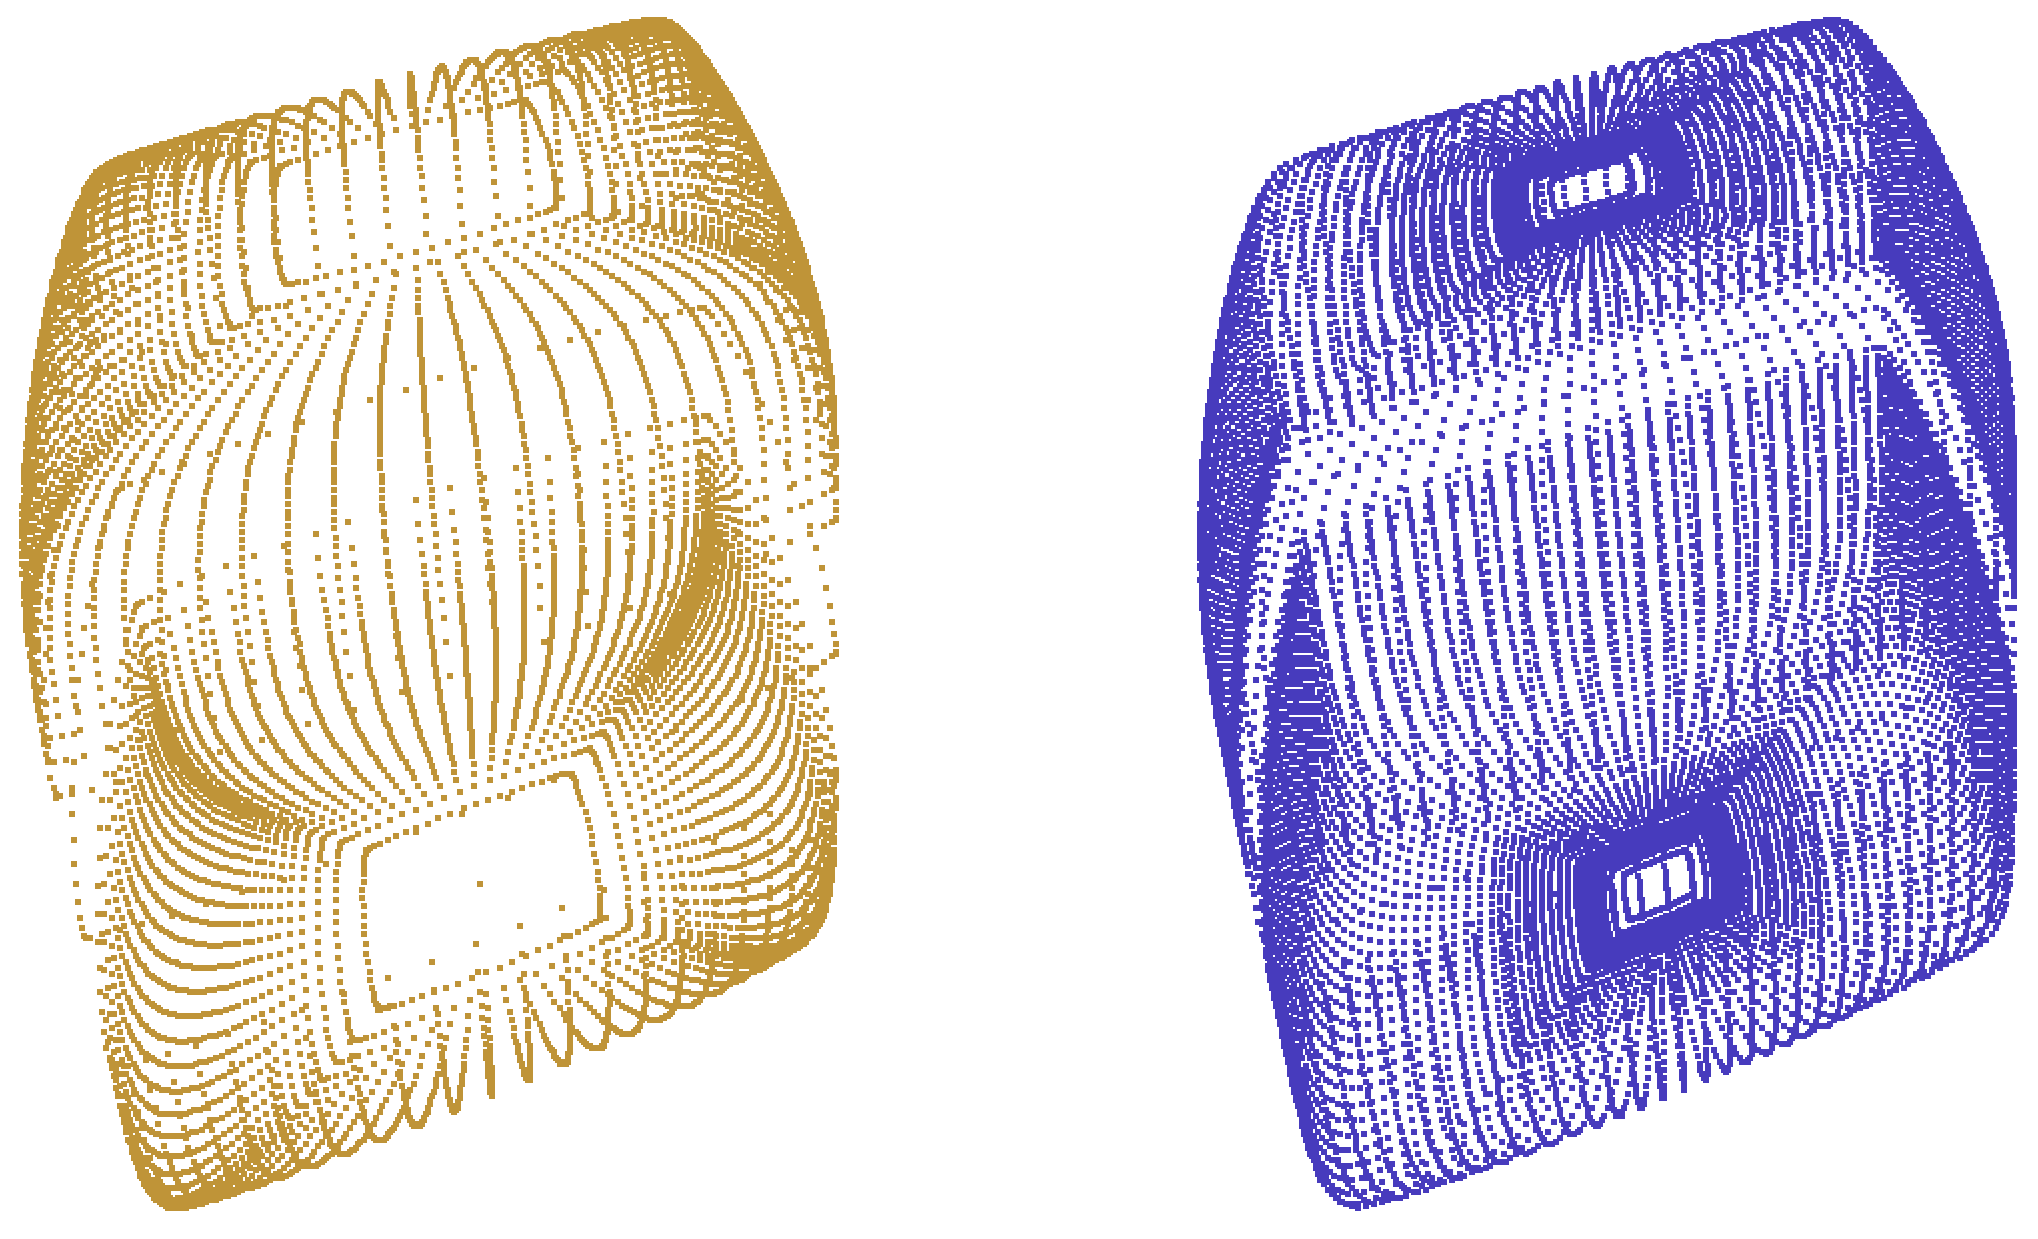
\includegraphics[width=0.75\columnwidth]{figures/sampling_smart_1}
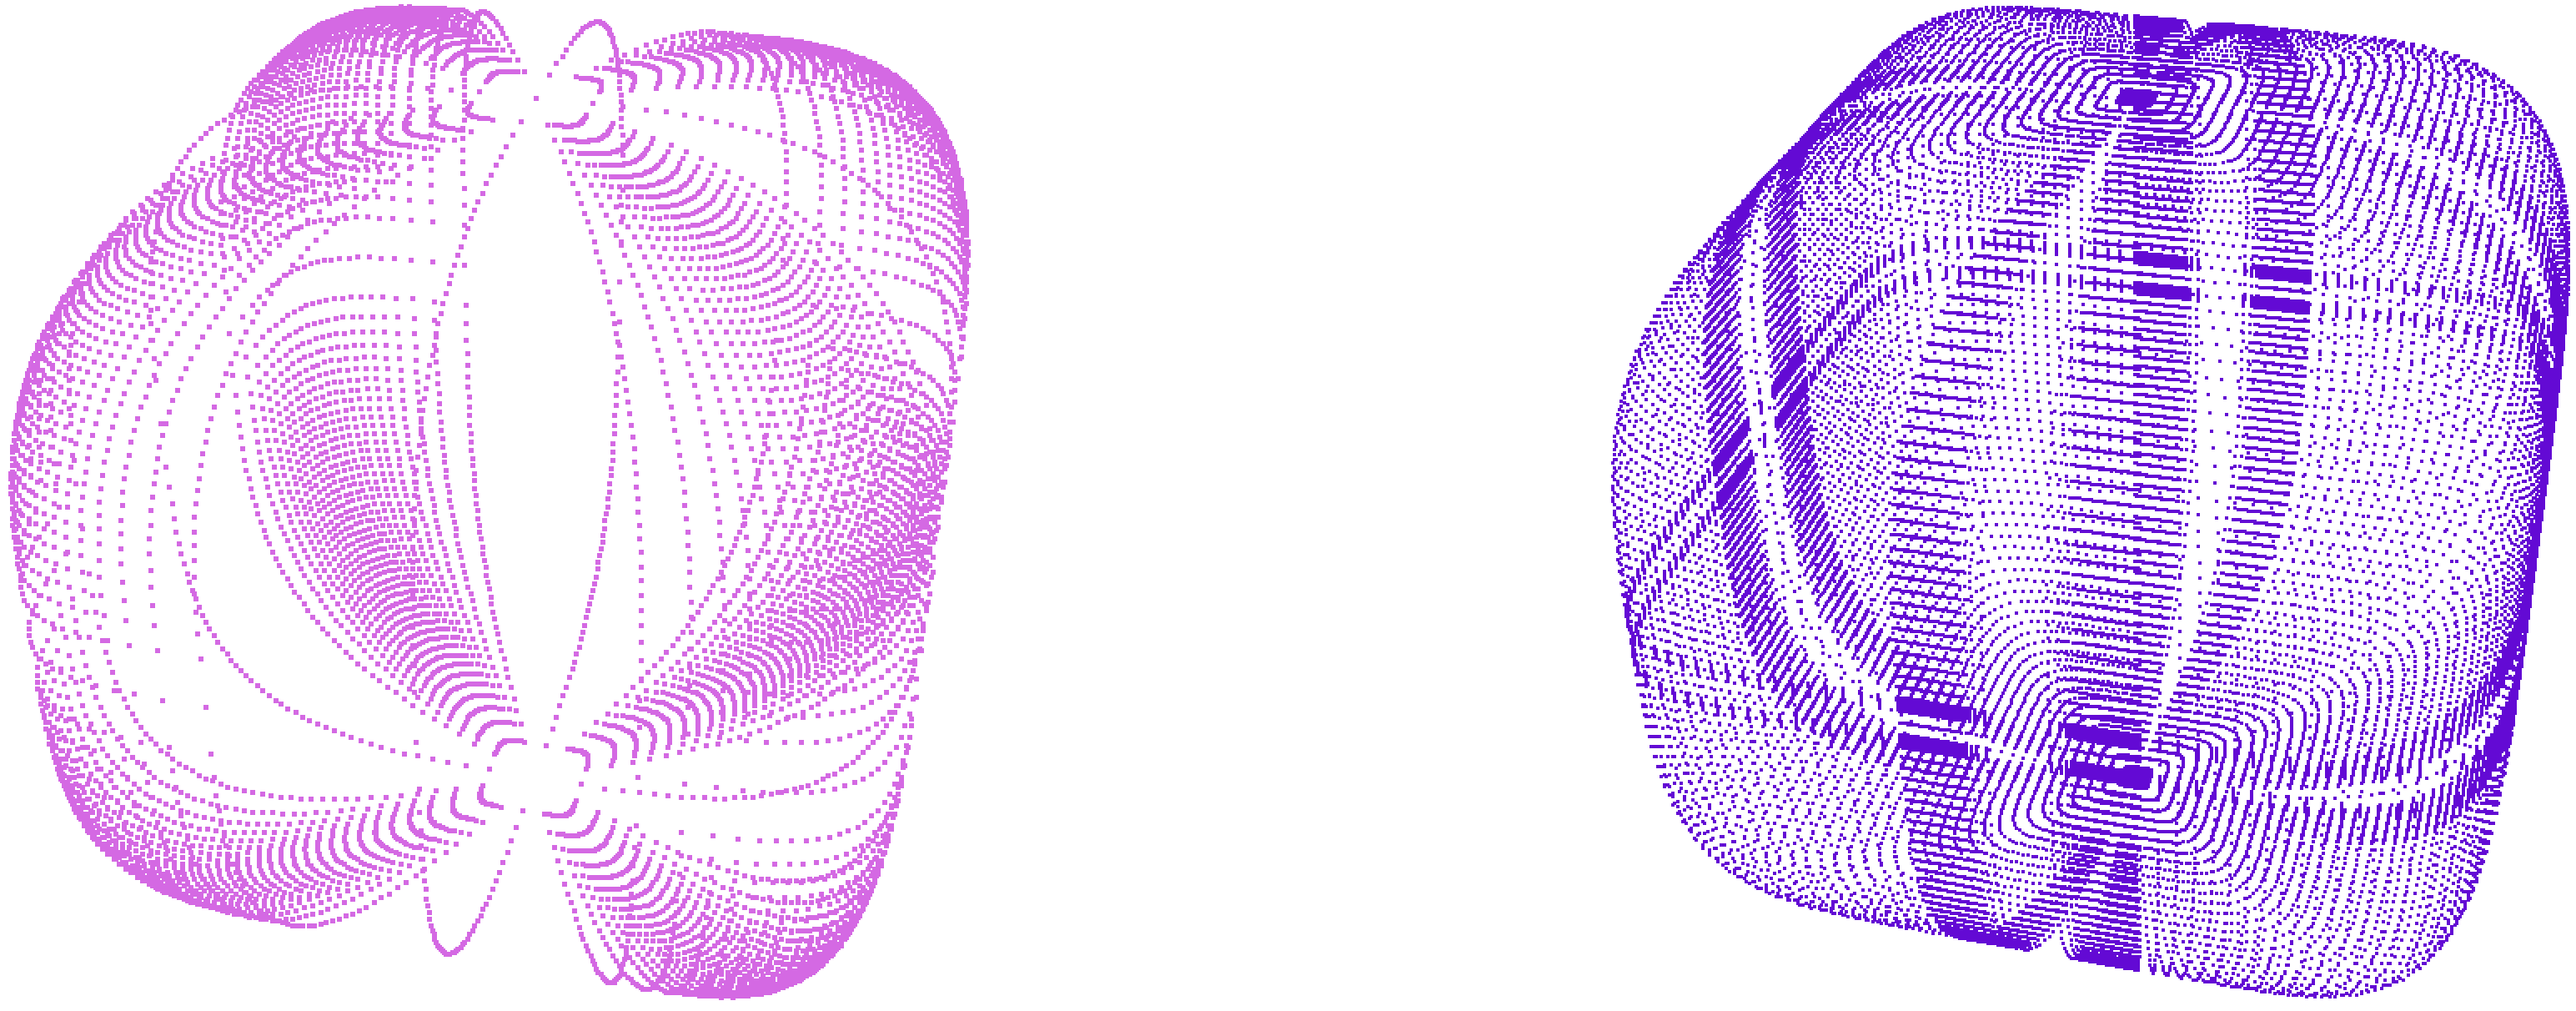
\includegraphics[width=0.75\columnwidth]{figures/sampling_smart_2}
\caption {Superquadric sampling by adapting the angular parameter sampling so that the 3D space is uniformly sampled.}
\label{fig:sampling_smart}
\end{figure}



%%%%%%%%%%%%%%%%%%%%%%%%%%%%%%%%%%%%%%%%%%%%%%%%%%%%%%%%%%%%
%%%%%%%%%%%%%%%%%%%%%%%%%%%%%%%%%%%%%%%%%%%%%%%%%%%%%%%%%%%%
\section {Fitting}
\label{sec:fitting}

\subsection*{Error functions}

One could simply use the implicit equation for fitting the superquadric models, but experiments show that the optimizer tends to converge to models that incorporate the given point set as a small part of their shape (i.e., very large solids). As such, \cite{SQ_2000} suggest to scale the error function by the square root of the product of the scales of the superquadric, in order to penalize large volumes. This technique is employed and confirmed by \cite{journals/pami/KatsoulasBK08}, \cite{conf/wscg/ChevalierJB03}. Observe that the additional $\epsilon_1$ exponent is used in order to have a correct distance measure independent of the shape parameter. In addition, \cite{conf/wscg/ChevalierJB03} suggest to use the radial Euclidean distance instead of the normal Euclidean distance (i.e., scale the Euclidean distance by $OP$, the distance between the point and the center of the superquadric).

\begin{equation}
min \sqrt {a_1 a_2 a_3} \sum_{k=0}^n ||OP|| * \left[ \left( \left( \left( \frac{x}{a_1}\right)^{\frac{2}{\epsilon_2}} + \left( \frac{y}{a_2} \right) ^{\frac{2}{\epsilon_2}} \right)^{\epsilon_2 / \epsilon_1} + \left( \frac{z}{a_3} \right) ^{2/\epsilon_1} \right) ^{\epsilon_1} - 1 \right]
\end{equation}


In our implementation, we first used the unstable branch of the Eigen library \cite{eigenweb} which contains a rough Levenberg Marquardt algorithm implementation. Due to its lack of customizability, we looked for better options. As such, we decided to use the CERES solver library \cite{ceres-solver}. This is a large library employed for applications such as Google Street View and Google Maps. It is essentially a portable C++ library that allows for modeling and solving large complicated nonlinear least squares problems.

At each iteration of the LM algorithm, it needs to compute the Jacobian matrix of the vector of variables. CERES allows for three options:

\begin{itemize}
	\item {using the explicit formula in the code. We employed Maple to generate the C code from the symbolic partial differentiation of the error function; this yielded good results.}
	\item {using numerical differentiation. Apart from the fact that it has to compute the error function twice, there are a lot of numerical stability problems due to the very large range of values involved in the calculation, straining the floating point representation past its limits.}
	\item {using the auto differentiation module of CERES. By using a special type named Jet, CERES is able to compute the symbolic derivatives of our expressions. Jet is an implementation of n-dimensional dual numbers. We decided to use this technique in the end, as it allows for quick and easy modifications of the error functions, and it yielded good performance.}
\end{itemize}

\subsection*{Initial fitting parameters}

Due to the presence of numerous local minima in the superquadric function landscape, we need to have a good initialisation for the optimizer. One immediate idea is to set the translation to be the center of the point set we are trying to fit the model into.

In addition, \cite{conf/icra/BiegelbauerV07} suggests that the initial solution pose for the superquadric fitting optimisation is obtained by aligning the z-axis of the superquadric with each of the 3 central moments of the point set (i.e., the 3 PCA decomposition axes). We then choose the fitting with the best error out of the 3.

Furthermore, \cite{xiao2005building} propose that $\epsilon_1$ and $\epsilon_2$ be initialised at their midrange values of 1 (considering that the range is $[0.1, 1.9]$). Similar to the previous paper, the orientation is to be set such that the axes of the superquadric are aligned to the principal axes of the data. Moreover, we assume that the point distribution on the principal axes is Gaussian, so we can initialise the 3 scale parameters of the superquadric to be 3 times the standard deviation of the points on each of the PCA axis (the square roots of the eigenvalues of the covariance matrix of the point set).

A set of results are visualised in Figure \ref{fig:fitting_results}.

\begin{figure}
\centering
\subfigure[]{
  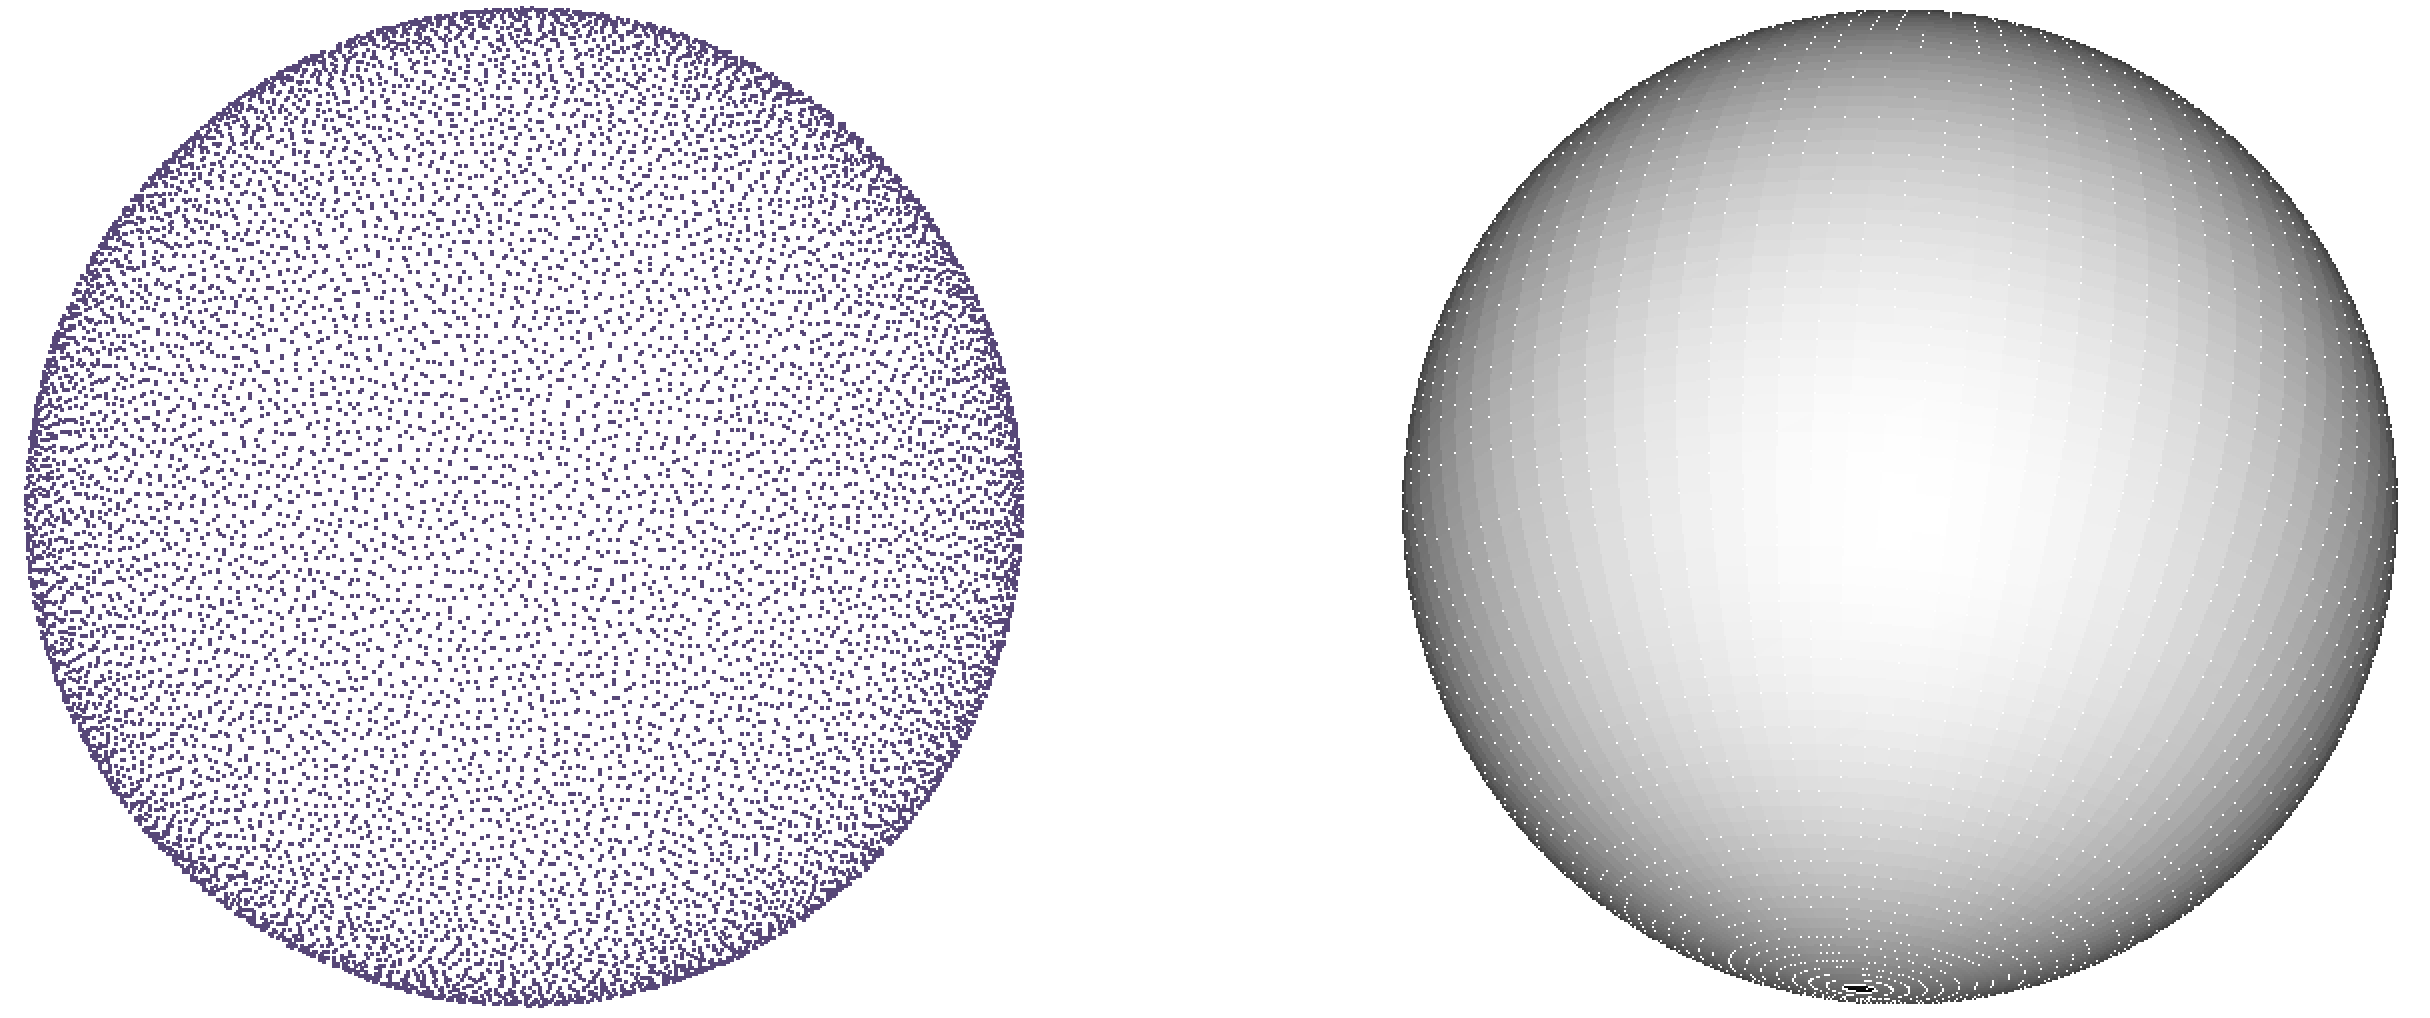
\includegraphics[width=0.45\columnwidth]{figures/fitting_example_1}} \\
\subfigure[]{
  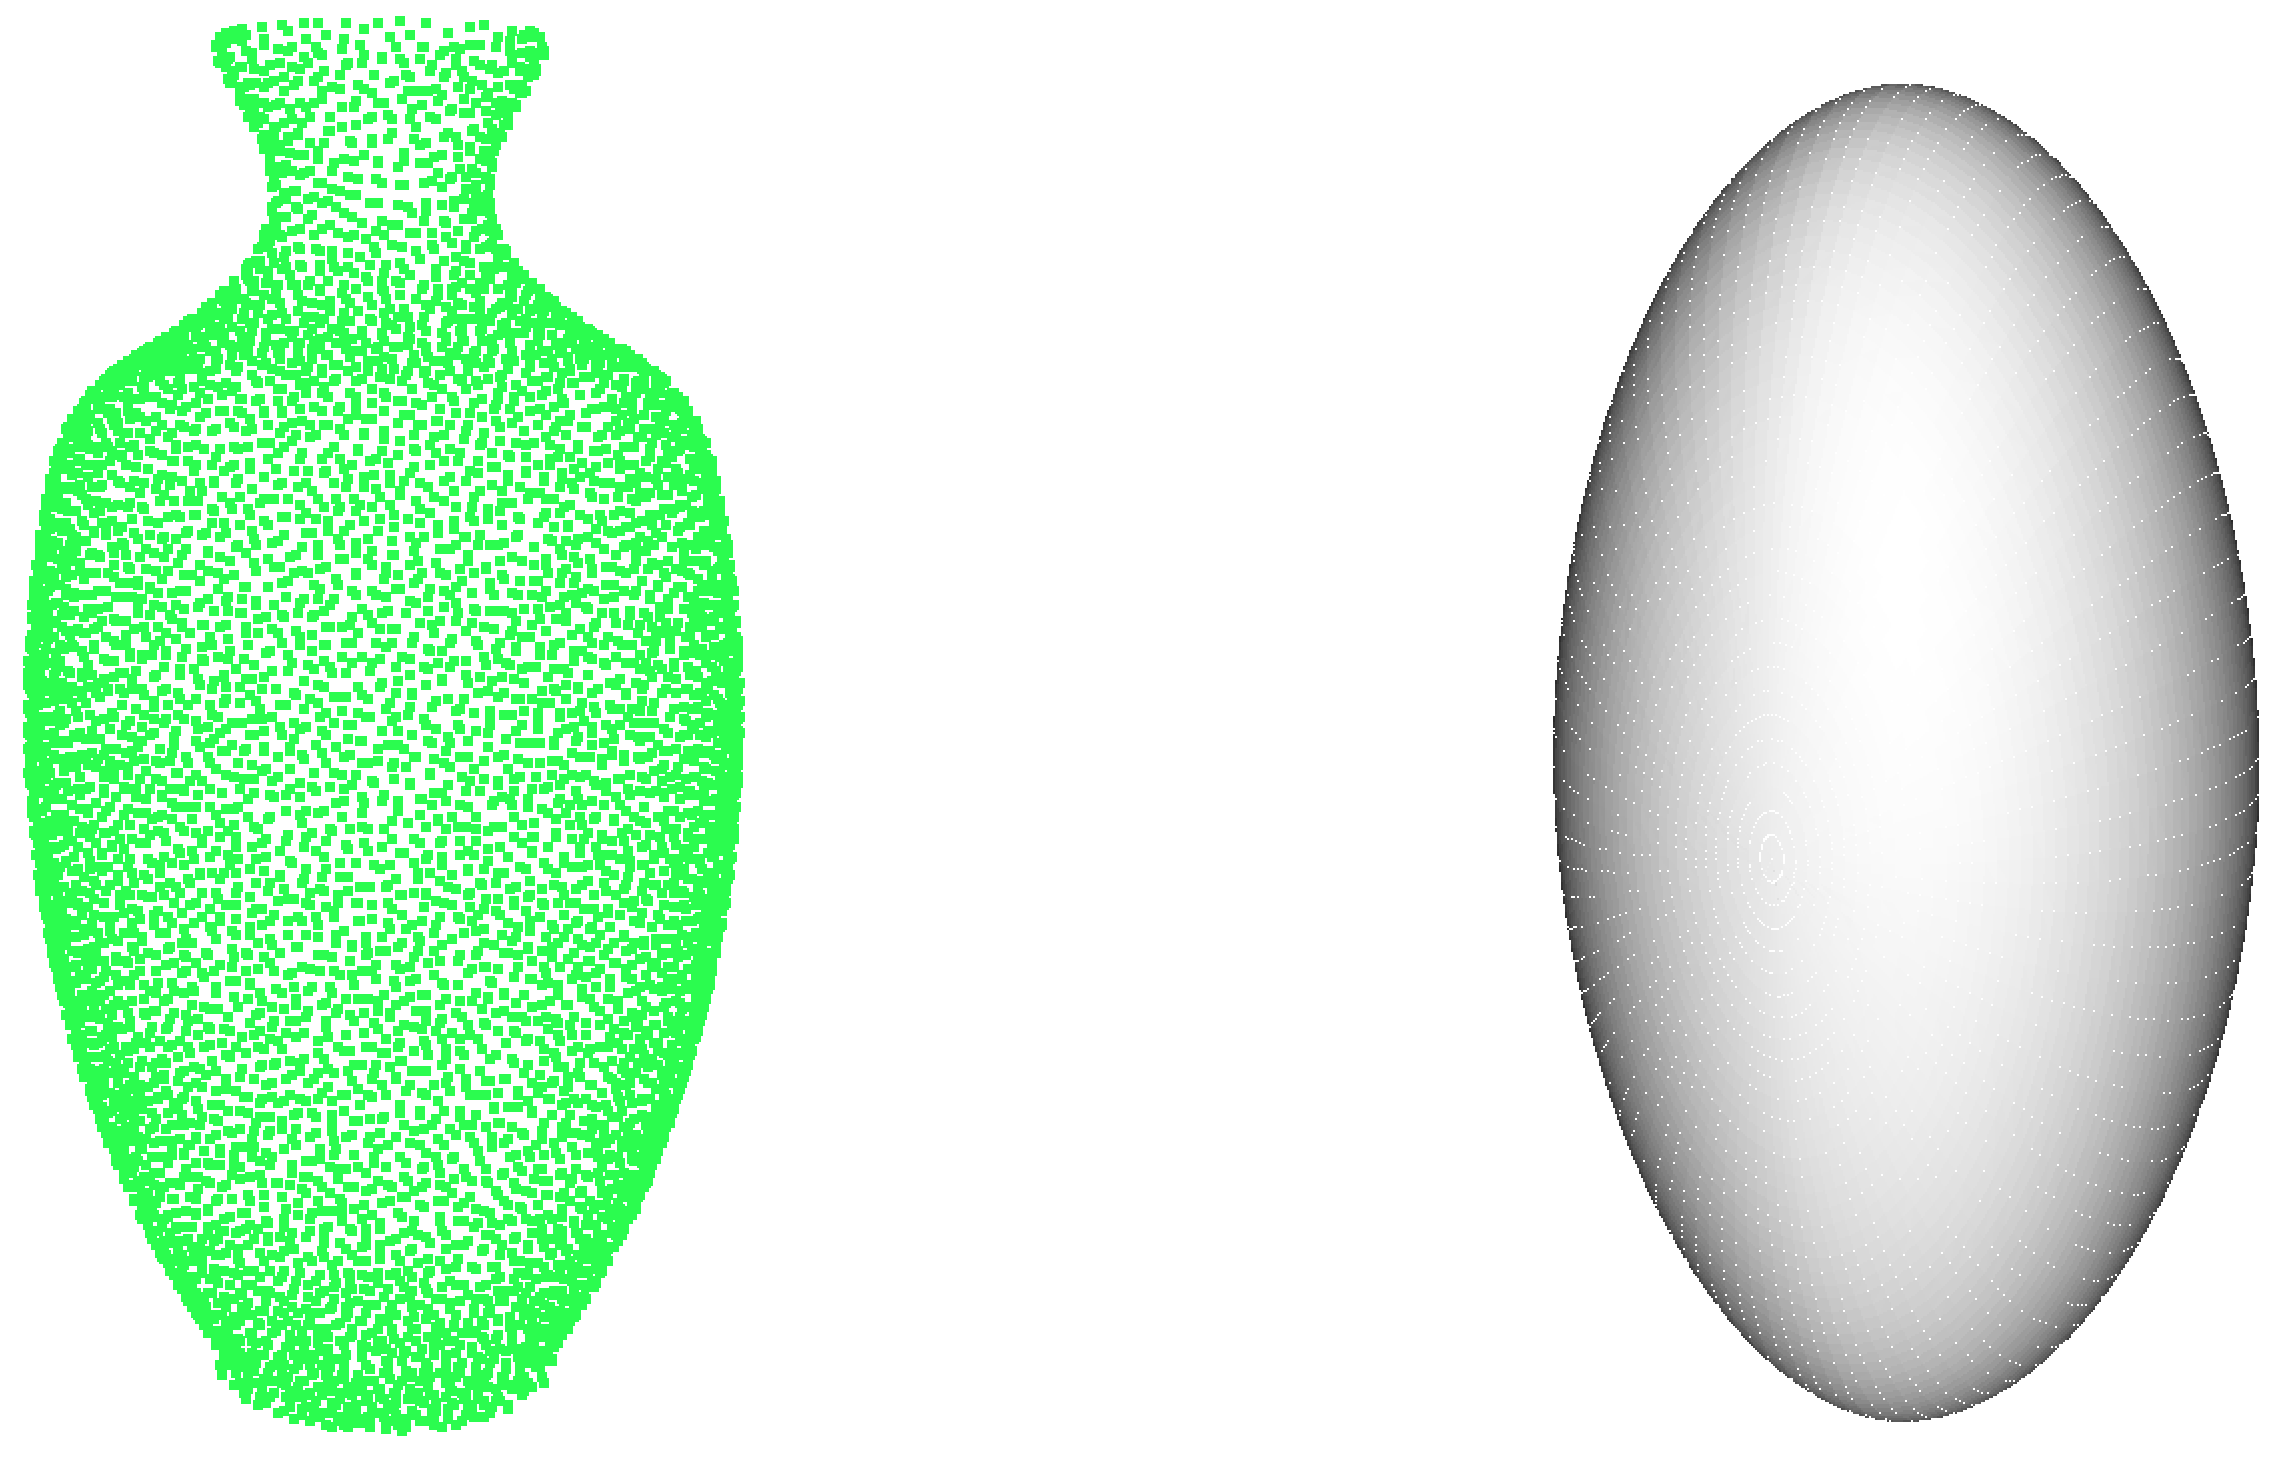
\includegraphics[width=0.45\columnwidth]{figures/fitting_example_2}} \\
\subfigure[]{
  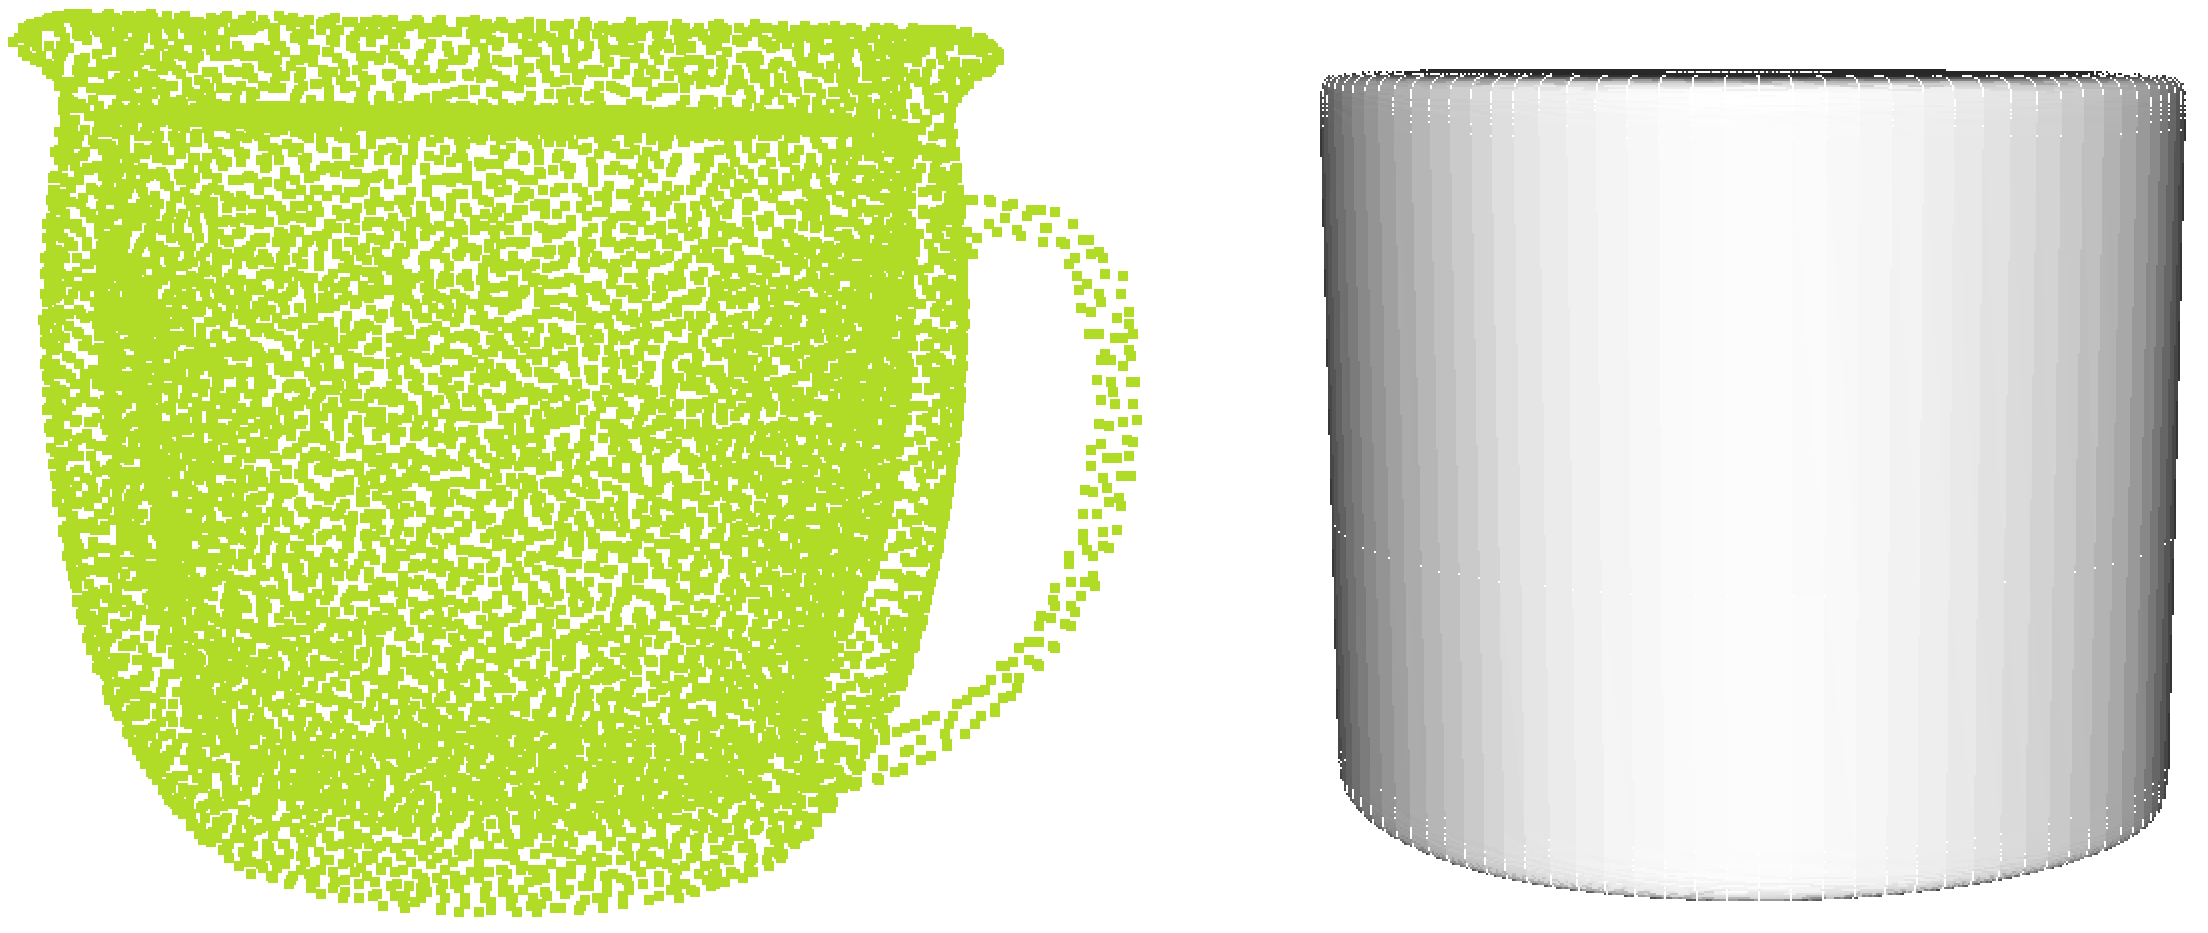
\includegraphics[width=0.45\columnwidth]{figures/fitting_example_3}} \\
\subfigure[]{
  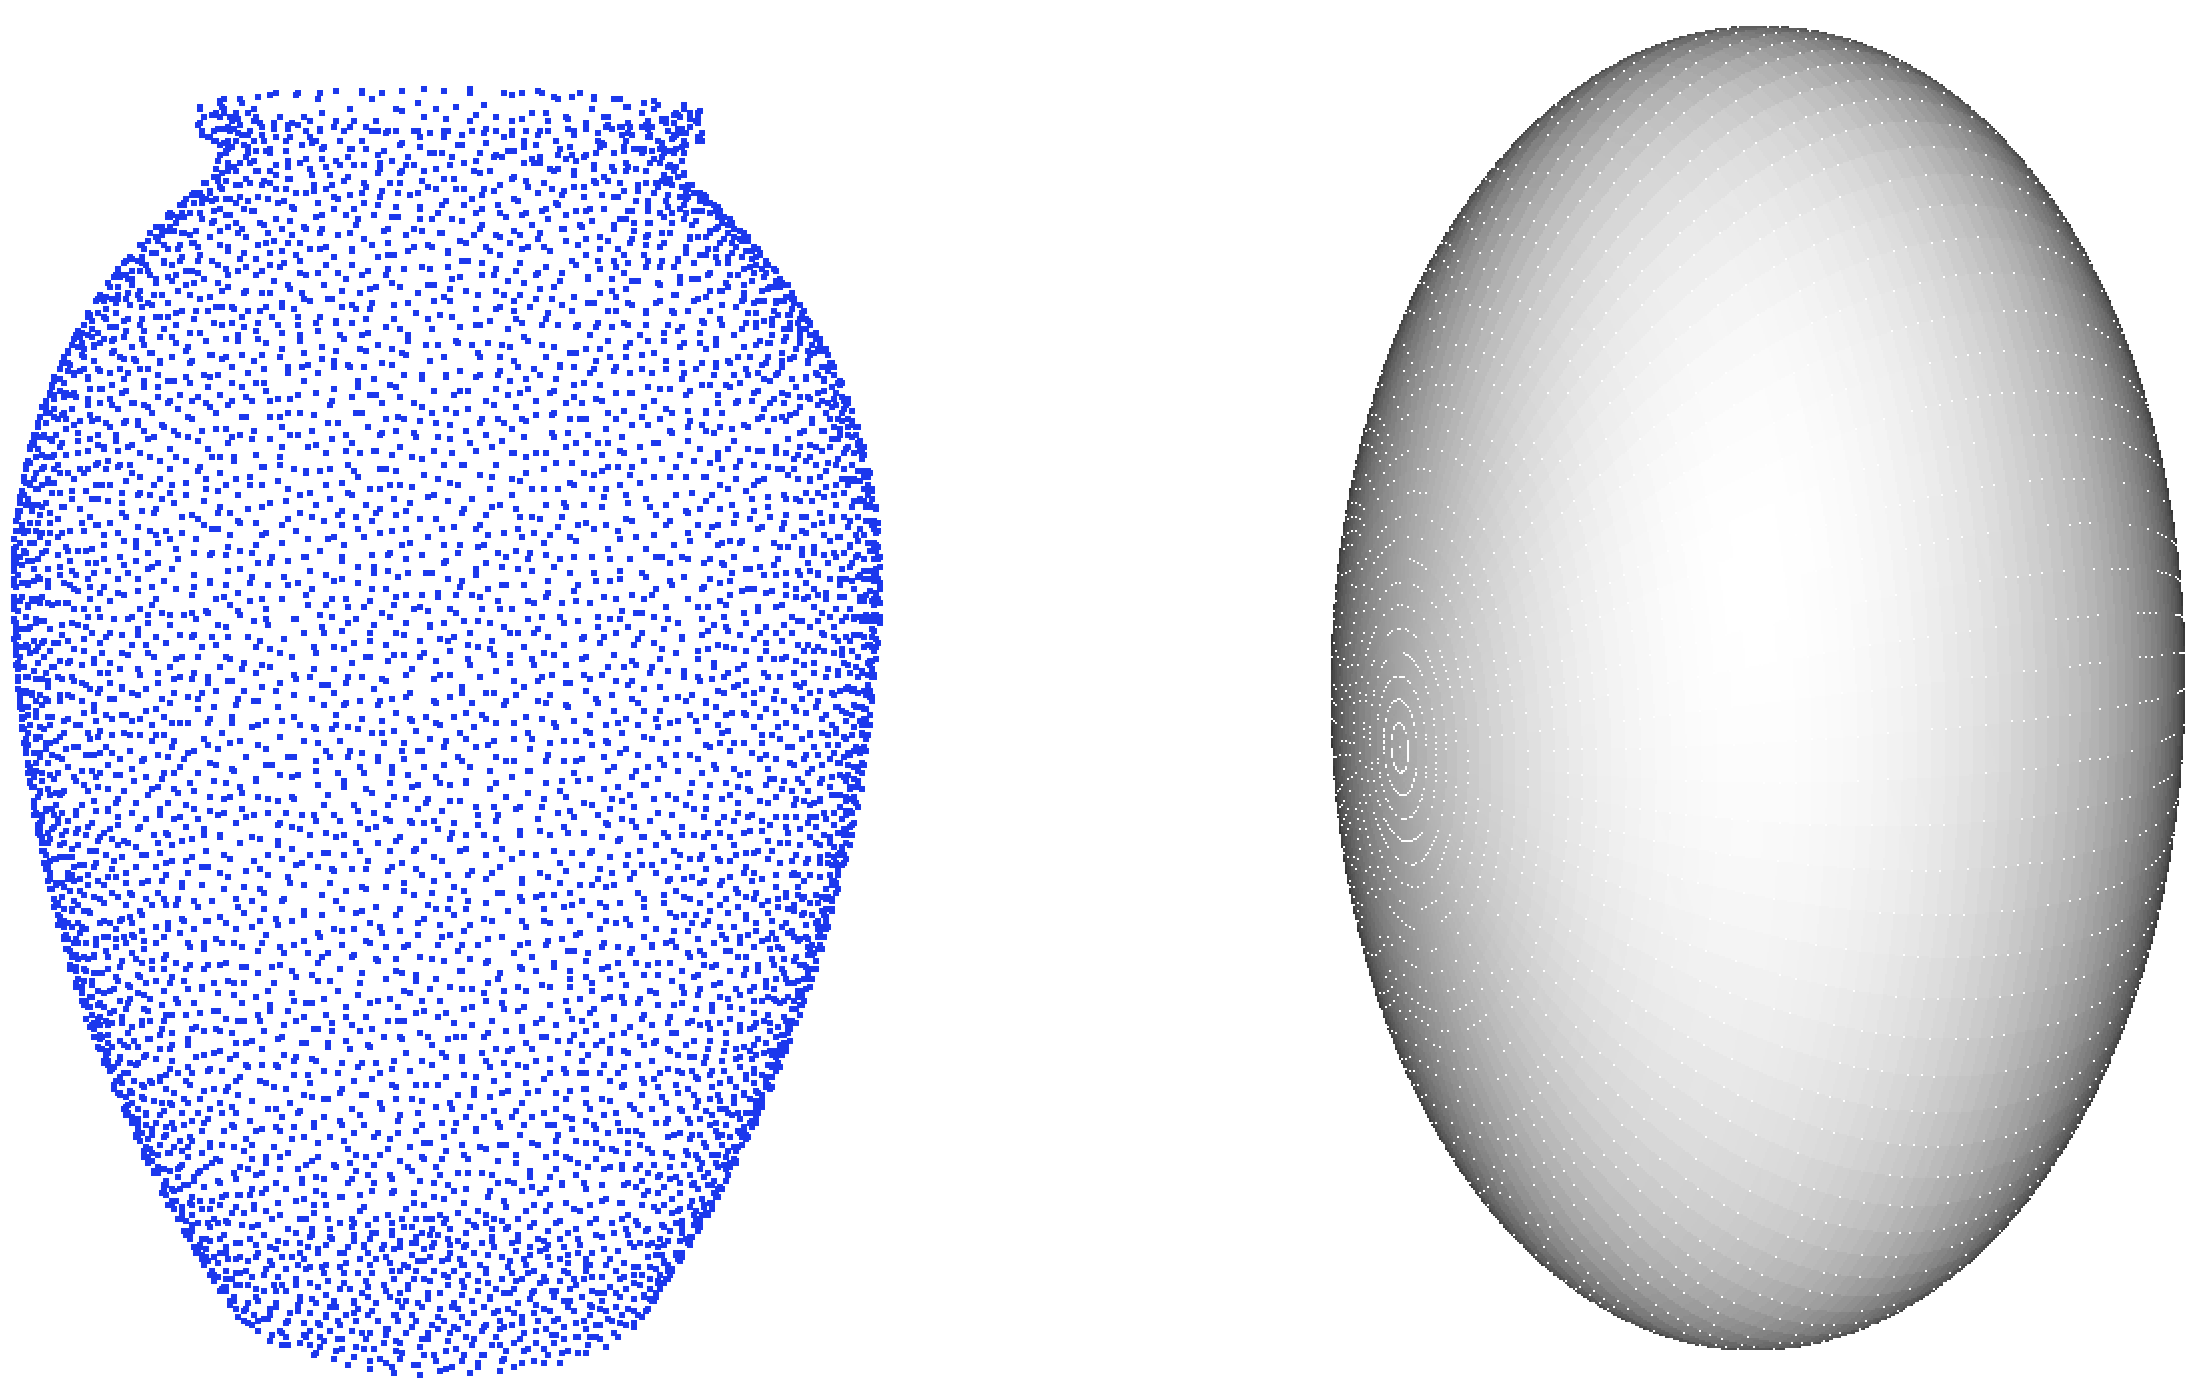
\includegraphics[width=0.45\columnwidth]{figures/fitting_example_4}}

\caption {Results of superquadric fitting on point clouds of complete single objects.}
\label{fig:fitting_results}
\end{figure}


\subsection {Multipart Fitting with a Split \& Merge Approach}

Another interesting direction we looked into is that of explaining a set of points by multiple superquadric models. \cite{doi:10.1117/1.1762516} propose a simple approach where a point set is segmented based on the local curvature, and then each cluster is fitted with a parametric model. Although the results presented in the paper looked reasonably good, we did not go for this technique (although we presented a similar per-cluster object fitting technique in Section \ref{sec:tabletop_demo}), as we foresaw possible robustness problems.

As a result, we found the split and merge approach of Chevalier et al. \cite{conf/wscg/ChevalierJB03} to be a better choice. \\

\textbf{Splitting}
\begin{itemize}
	\item {fit a superquadric to the current set of 3D points}
	\item {if the fitting error is less than a threshold $T$, then we stop (i.e., this cluster is well fitted to a superquadric)}
	\item {otherwise, the set of points is split in two regions, by cutting it with the plane orthogonal to the principal axis of the point set and going through the centroid of the points.}
	\item {the procedure is then called recursively on each half-subset until the number of points is too small for the cluster to be split again.}
\end{itemize}

\textbf{Merging}
\begin{itemize}
	\item {for each subset of points, determine its list of neighboring subsets. (*)}
	\item {try to merge the subset with each of its neighbors, choosing the merge that has a fitting error below a threshold $T'$ and the volume of the new superellipsoid is smaller than the sum of the volumes of the two superellipsoids fitted in the cluster before.}
	\item {re-iterate until no more merges are done.}
\end{itemize}

(*) - the original paper does not explain how the neighbouring subsets are found. We employ a simple technique to solve this issue: when doing the splitting, we store all the separating planes. Two subsets are considered to be neighbouring if the segment connecting the centroids intersects less than 3 splitting planes.

Figure \ref{fig:split_merge} shows a few results we got by using this algorithm on synthetic data. We tested this technique on real datasets, but with no good results, as it is very sensitive to incomplete data. But it seems to work fairly well on complete CAD models. Further testing should be done here with full 360 degrees KinFu scans.

\begin{figure}
\centering
\subfigure[]{
  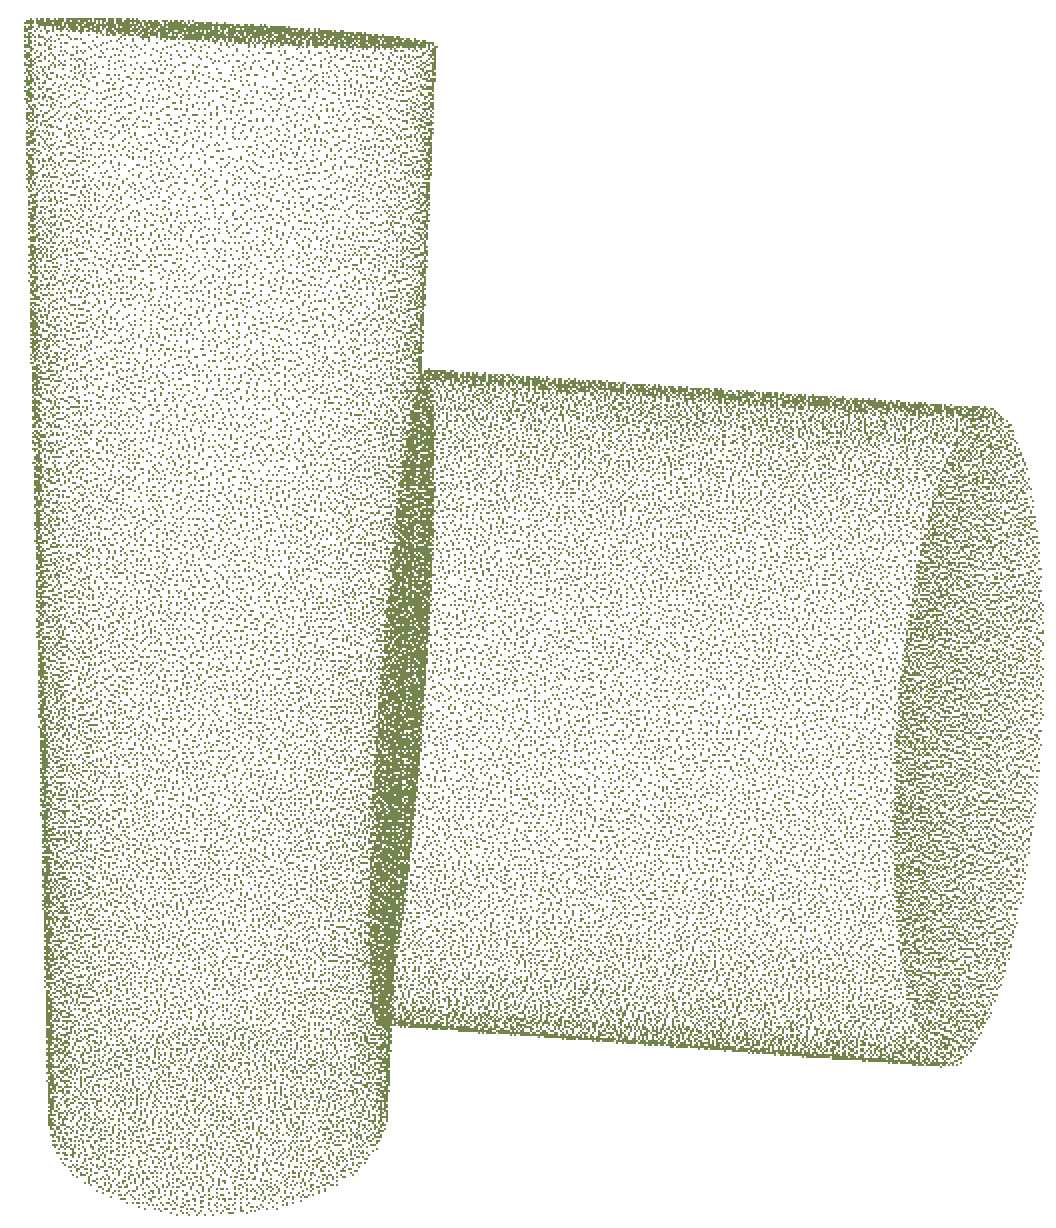
\includegraphics[width=0.3\columnwidth]{figures/2_components_cloud}}
\subfigure[]{
  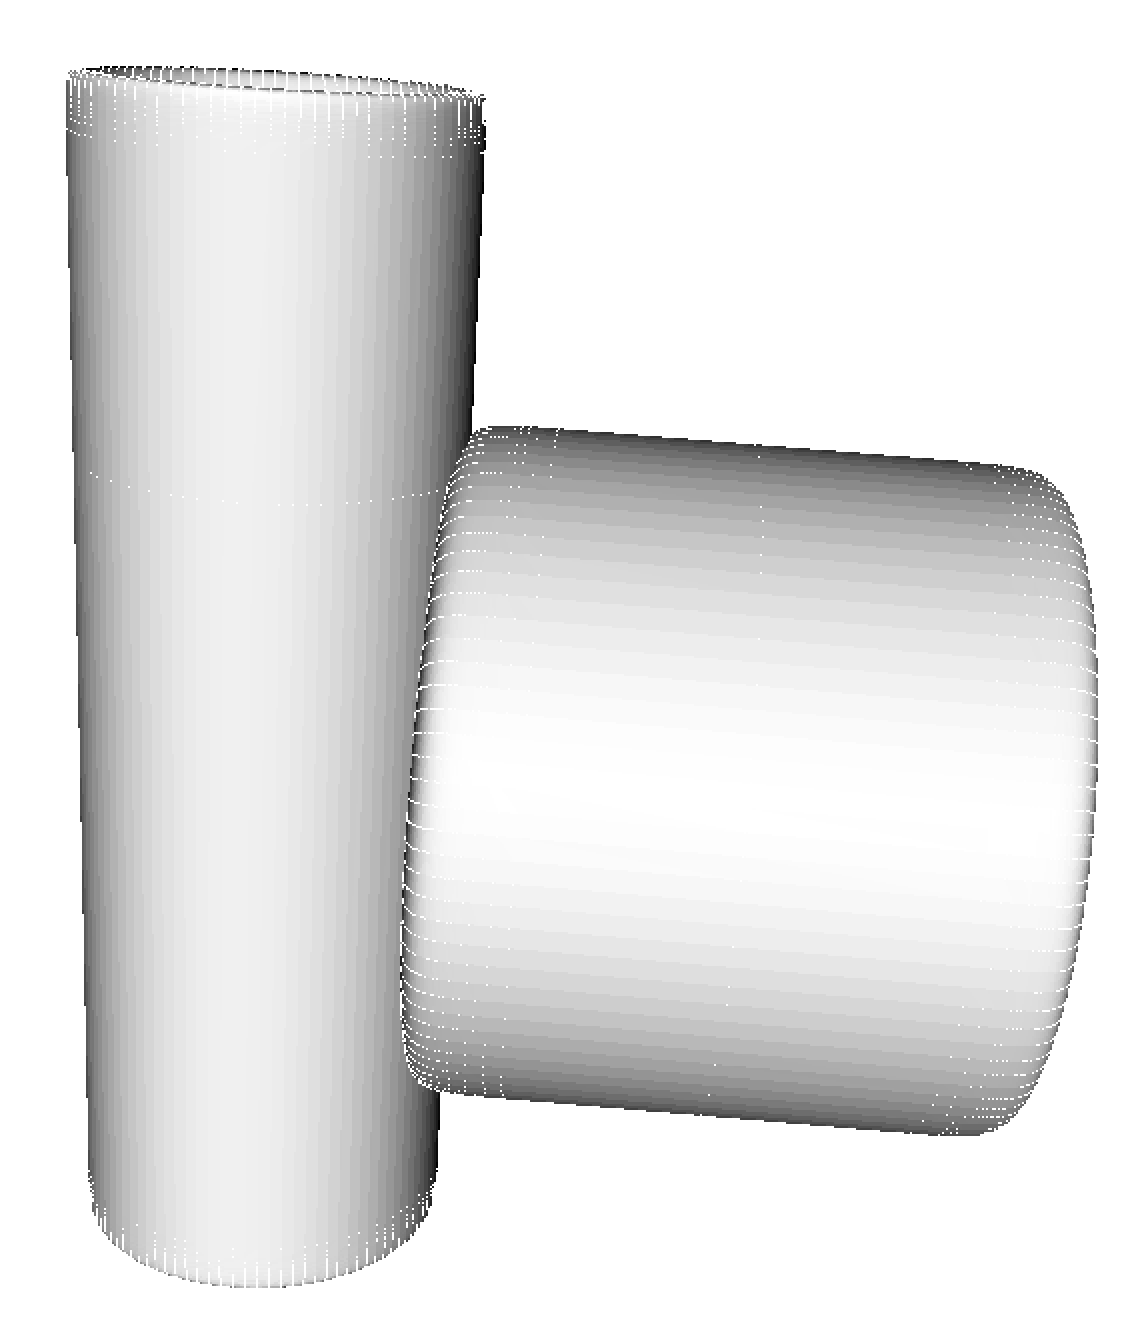
\includegraphics[width=0.3\columnwidth]{figures/2_components_fitted}}

\subfigure[]{
  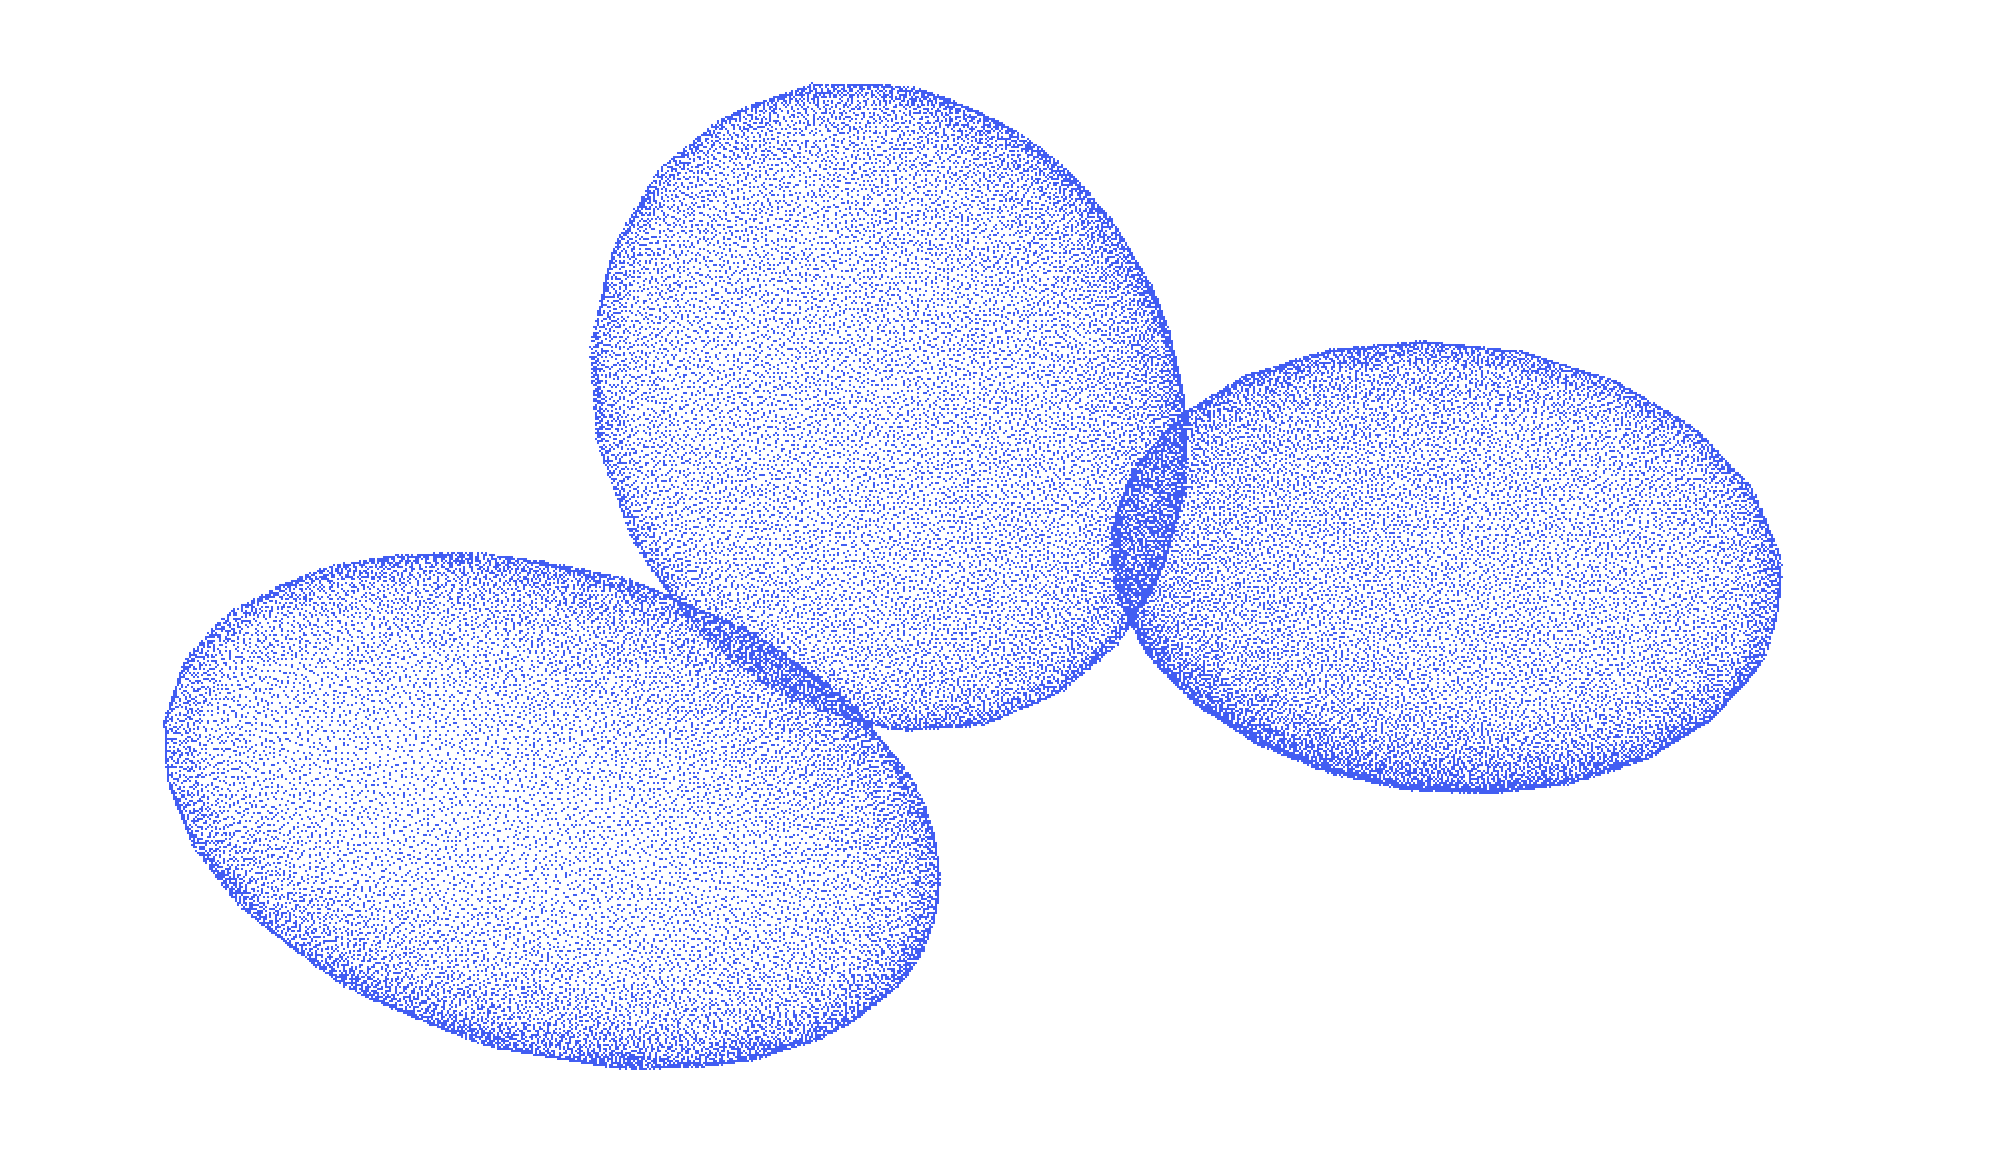
\includegraphics[width=0.45\columnwidth]{figures/3_ellipsoids_cloud}}
\subfigure[]{
  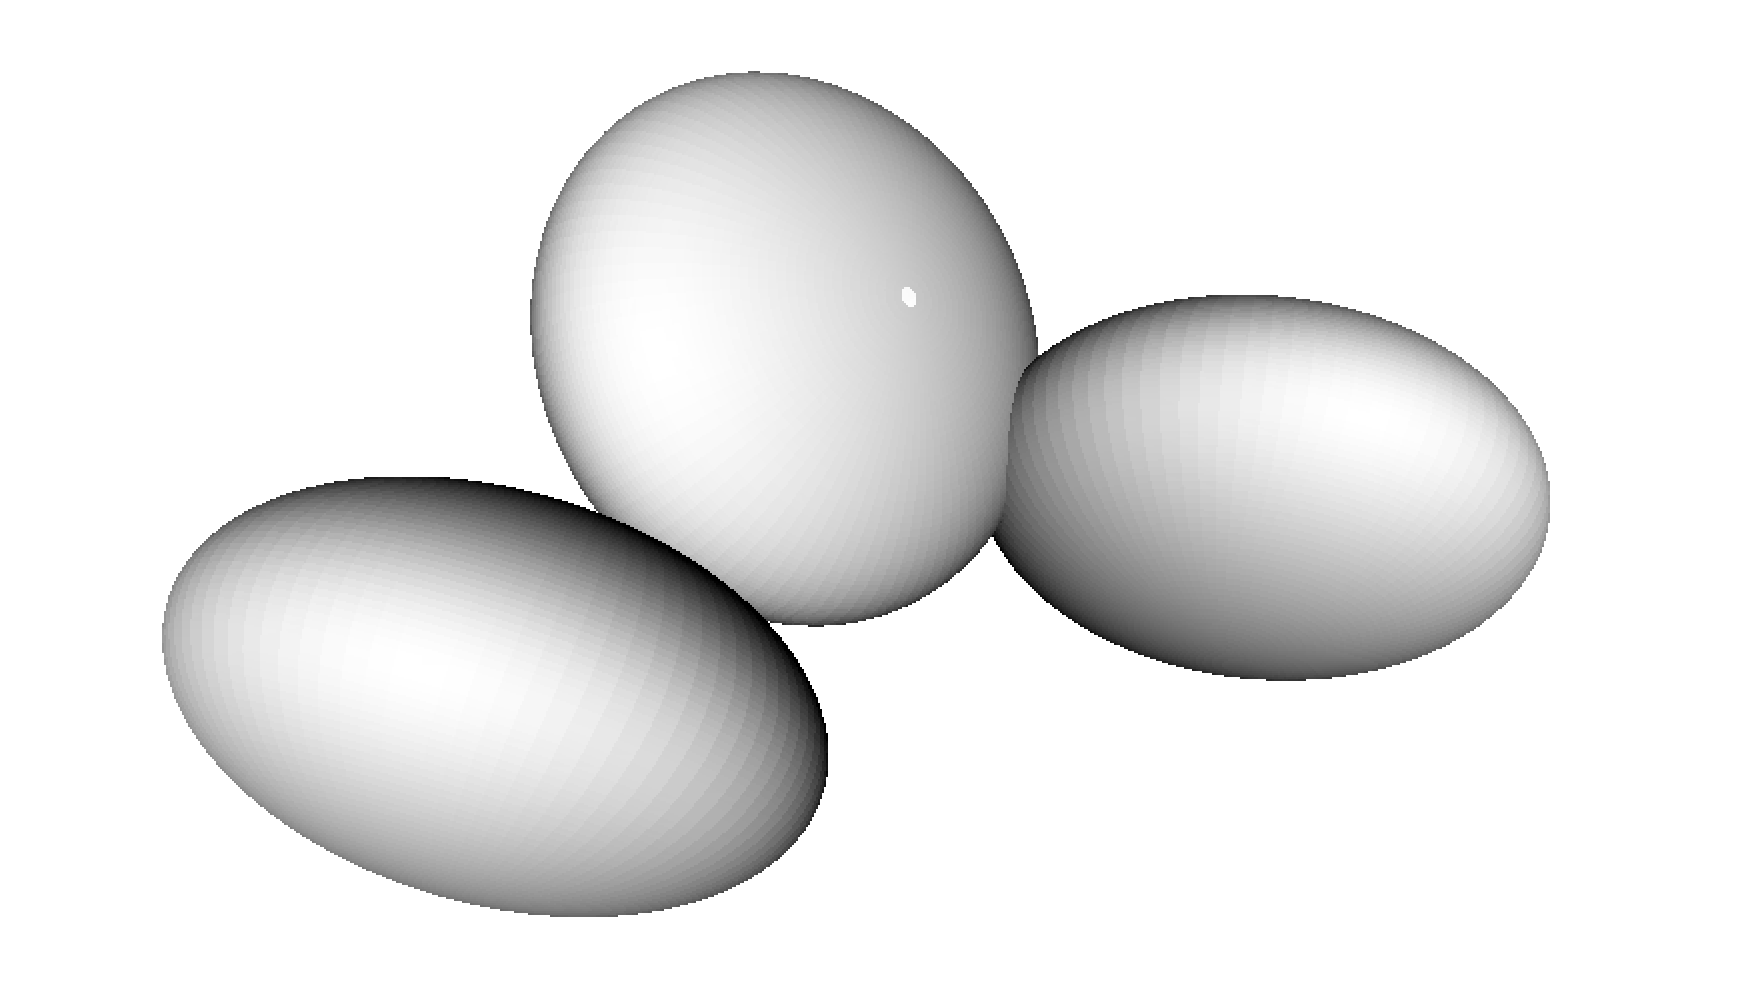
\includegraphics[width=0.45\columnwidth]{figures/3_ellipsoids_fitted}}

\caption {Split and merge algorithm results.}
\label{fig:split_merge}
\end{figure}




\section {Detection}
\label{sec:detection}

One of most popular techniques for detecting parametrized models in point cloud scenes is RANSAC \cite{fischler1981random}. Superquadric object detection has been tackled in \cite{afanasyev3d}, \cite{conf/caip/KrivicS01}, and \cite{conf/icra/BiegelbauerV07}, and we considered that the approach of Biegelbauer et al. \cite{conf/icra/BiegelbauerV07} had the most convincing results and we implemented it.

Figure \ref{fig:superquadric_detection_schematic} shows the general idea behind Biegelbauer's solution. The first step is to preprocess the data by removing the largest plane and possibly segmenting clusters of points that might represent separate objects in order to ease the detection process. Next, we generate $m$ hypotheses by selecting $m$ ($\sim 20$) random seed points from the scene. Then, we find the points in the neighbourhood of the seed point of size equal to the minimum scaling parameter of the superquadric we are looking for ($min (a_1, a_2, a_3)$). Inside this small set of points, we randomly choose 30 points and try to rigidly align the superquadric we are looking for. We repeat this process $ransac\_restarts$ times ($\sim 10$) and choose the best fitting pose. This pose is then used as an initialisation for a fitting procedure that includes all the points in the neighborhood. We then compute the fitting error and the number of interior and surface points to the parametric model within a neighbourhood of size $1.2 * max(a,b,c)$ around the center of the superquadric. All the possible poses are ranked by the fitting error, number of surface and interior points and the one which has the lowest sum of ranks is chosen as the output.

\begin{figure}
\centering
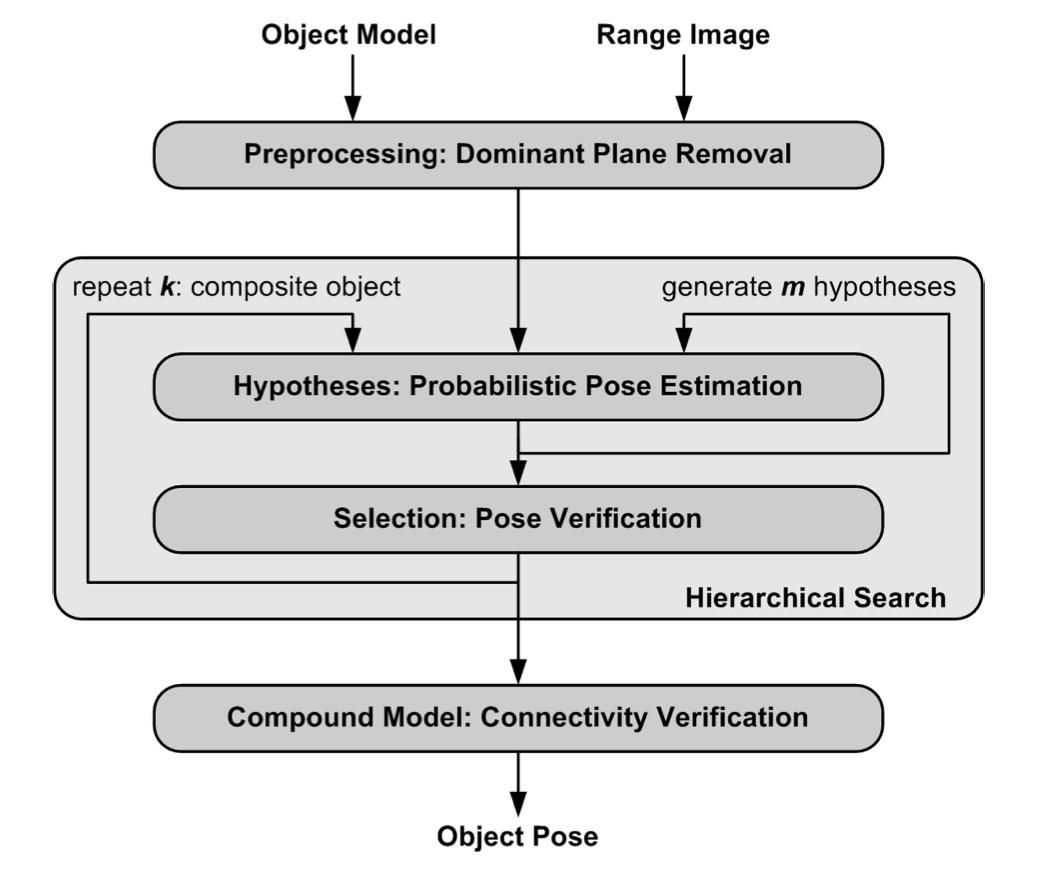
\includegraphics[width=0.55\columnwidth]{figures/superquadric_detection_schematic}

\caption{Superquadric detection pipeline as proposed by Biegelbauer et al. \cite{conf/icra/BiegelbauerV07}.}
\label{fig:superquadric_detection_schematic}
\end{figure}

One needs to note that finding the pose of a given superquadric inside a set of points is done similarly to the superquadric fitting presented in Section \ref{sec:fitting}, but only the 6 parameters for the pose are allowed to vary. However, we use the same initialisation techniques based on the principal axes of the point set.

\section {Tabletop Demo}
\label{sec:tabletop_demo} 

In order to demonstrate the superquadric algorithms we implemented on real world datasets, we have put together a pipeline for processing RGB-D data:

\begin{enumerate}
\item {Scan a scene for a few seconds (with an Asus Xtion Pro RGB-D camera) and register the frames using PCL KinFu. The input of the next stages is the point cloud obtained from the vertices of the 3D accumulation grid of KinFu.}
\item {Find the largest plane using RANSAC on the whole cloud.}
\item {Perform Euclidean clustering on the points that were identified to lie in the plane in order to find the largest continuous surface and discard the other points, and recompute the plane equation.}
\item {Project the planar points onto the plane and compute the concave hull in 2D. Simplify the 2D contour to a polygon with a few vertices.}
\item {(Optional) Filter the non-planar points by discarding the ones that are not above/below the plane polygon (i.e., their projection onto the plane does not lie within the 2D polygon).}
\item {With the non-planar points, do Euclidean clustering again in order to separate different objects.}
\end{enumerate}

A couple of example results of this procedure can be seen in Figure \ref{fig:tabletop_segmentation}.

\begin{figure}
\centering
 \subfigure[]{
  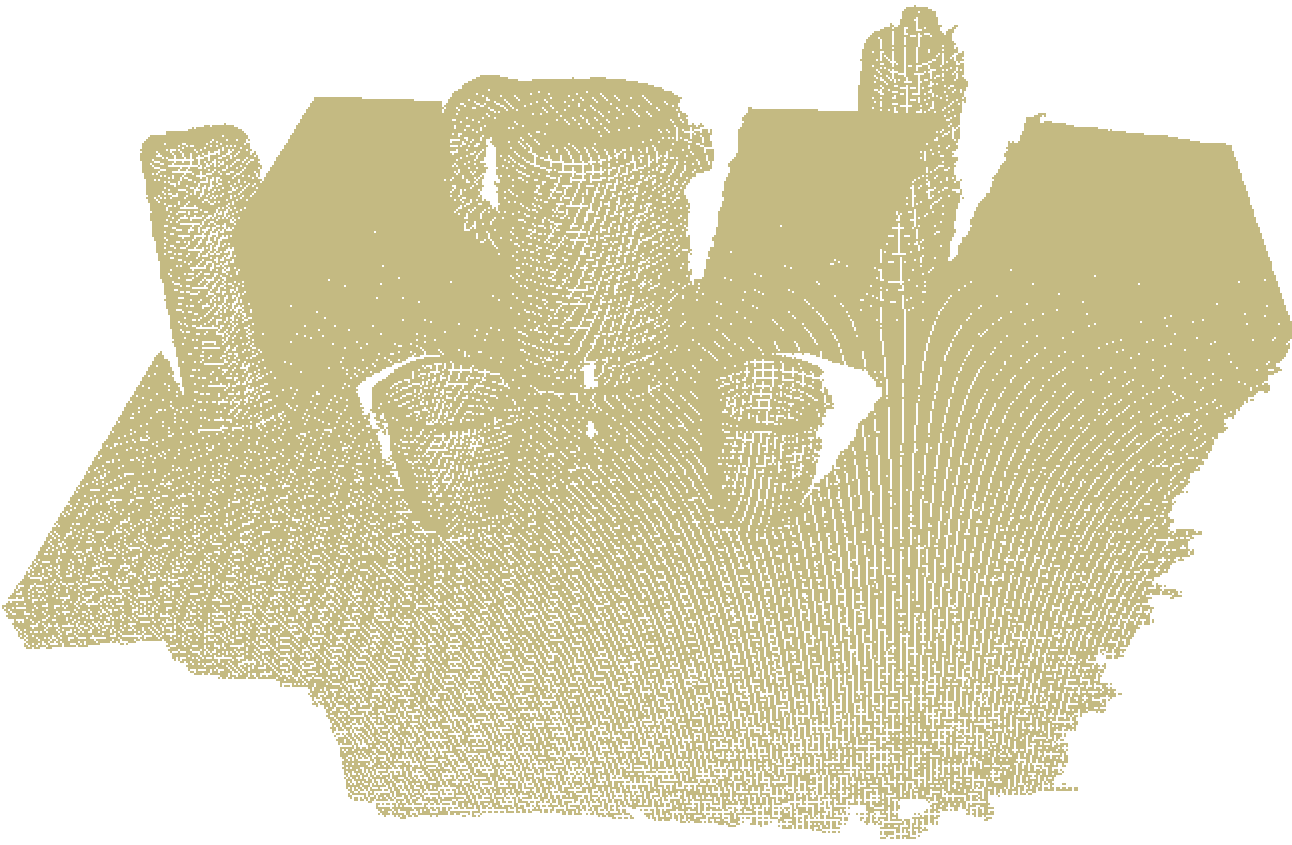
\includegraphics[width=0.45\columnwidth]{figures/segmentation_1_before}}
 \subfigure[]{
  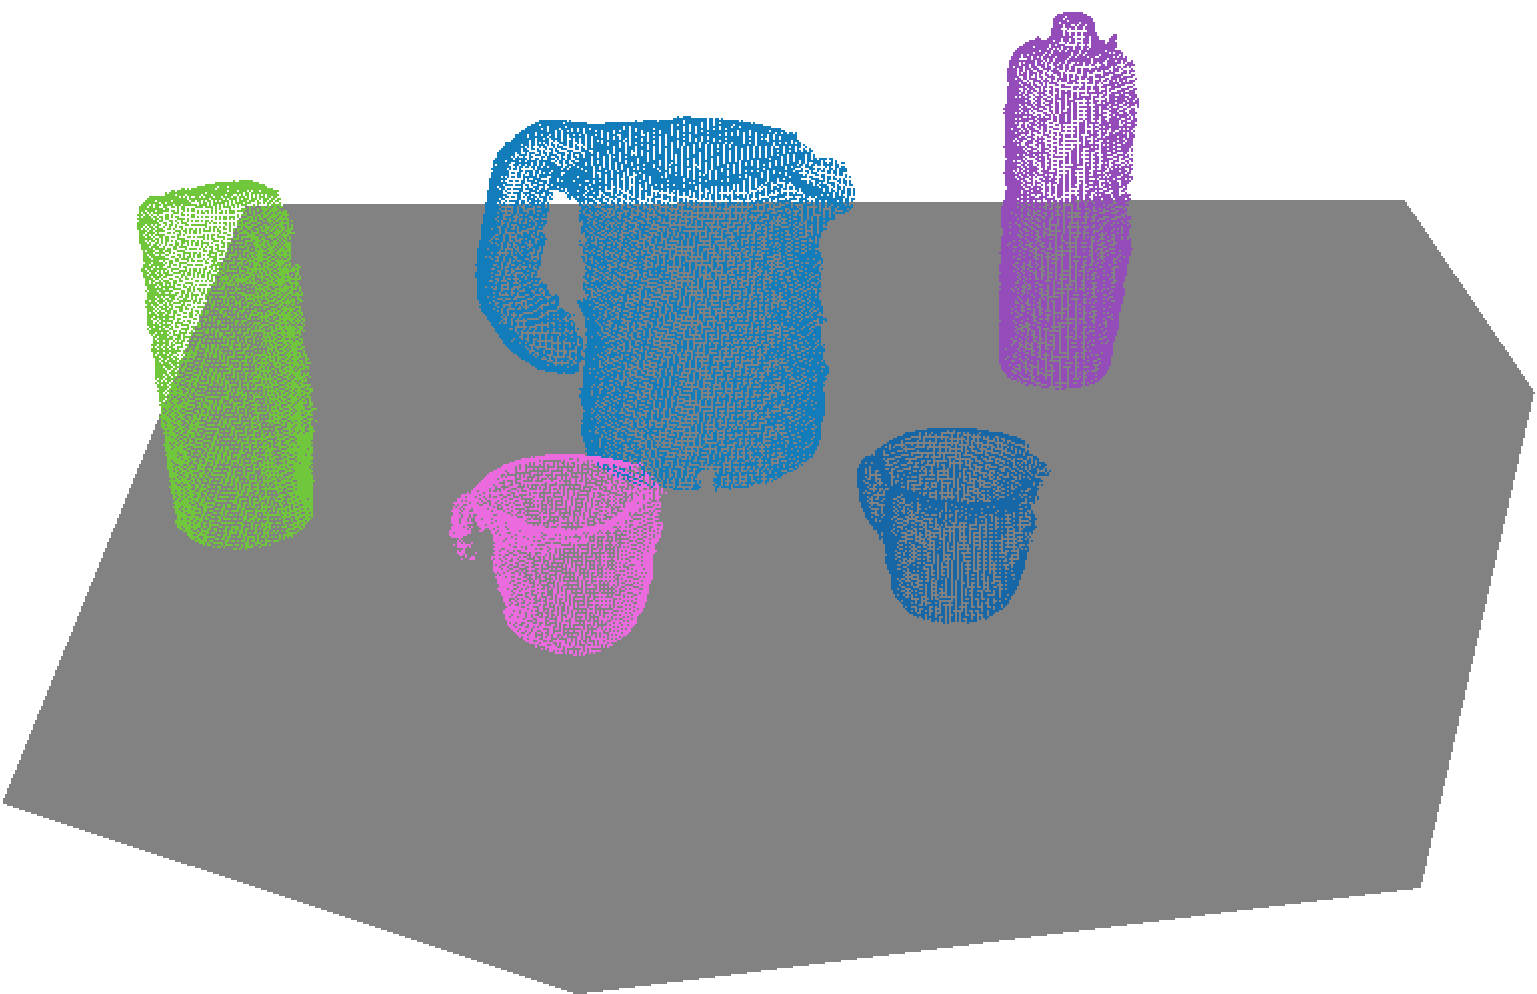
\includegraphics[width=0.45\columnwidth]{figures/segmentation_1_after}}
 \subfigure[]{
  
\includegraphics[width=0.45\columnwidth]{figures/segmentation_2_before}}
 \subfigure[]{
  
\includegraphics[width=0.45\columnwidth]{figures/segmentation_2_after}}

\caption{Our proposed tabletop segmentation: (a, c) the input cloud; (b, d) the output: the planar polygon and the separate object clusters that can be further processed.}
\label{fig:tabletop_segmentation}
\end{figure}

With the segmented data, we proceed in two directions: one is to fit a superquadric object to each separate cluster and one is to locate an object given its superquadric parametric description.

\subsection*{Superquadric fitting in real RGB-D data}
Figure \ref{fig:rgbd_fitting} shows the results we got and Table \ref{table:rgbd_fitting_timing} the time performance of our implementation.

\begin{figure}
\centering
 \subfigure[]{
  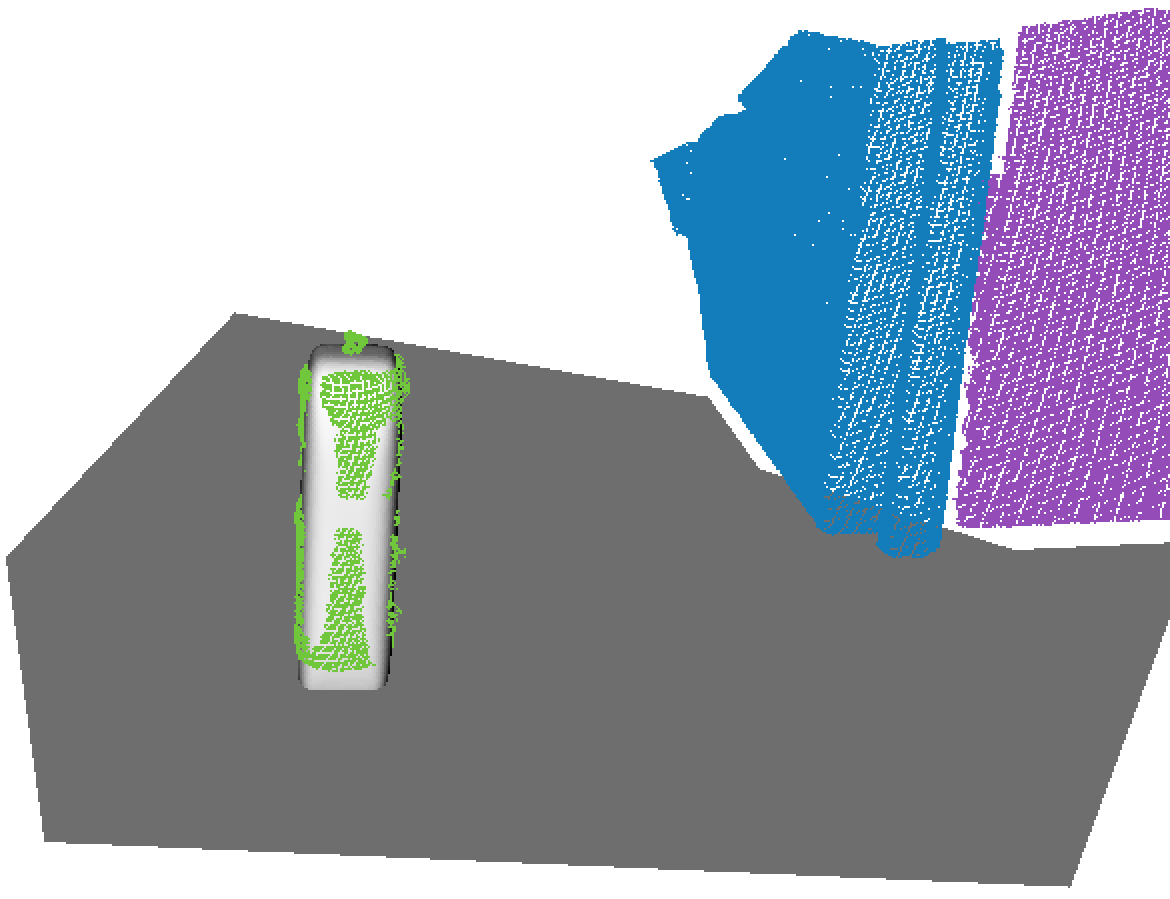
\includegraphics[width=0.45\columnwidth]{figures/rgbd_fitting_1}}
 \subfigure[]{
  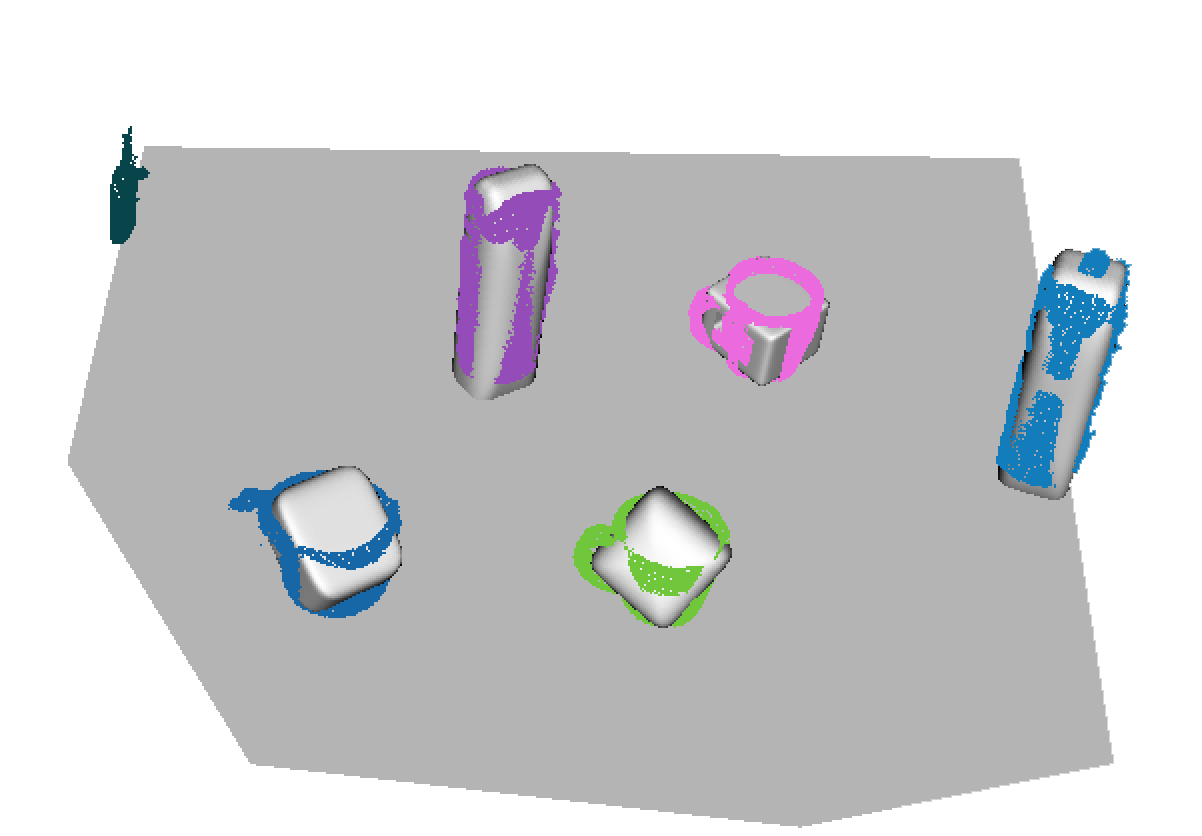
\includegraphics[width=0.45\columnwidth]{figures/rgbd_fitting_2}}
 \subfigure[]{
  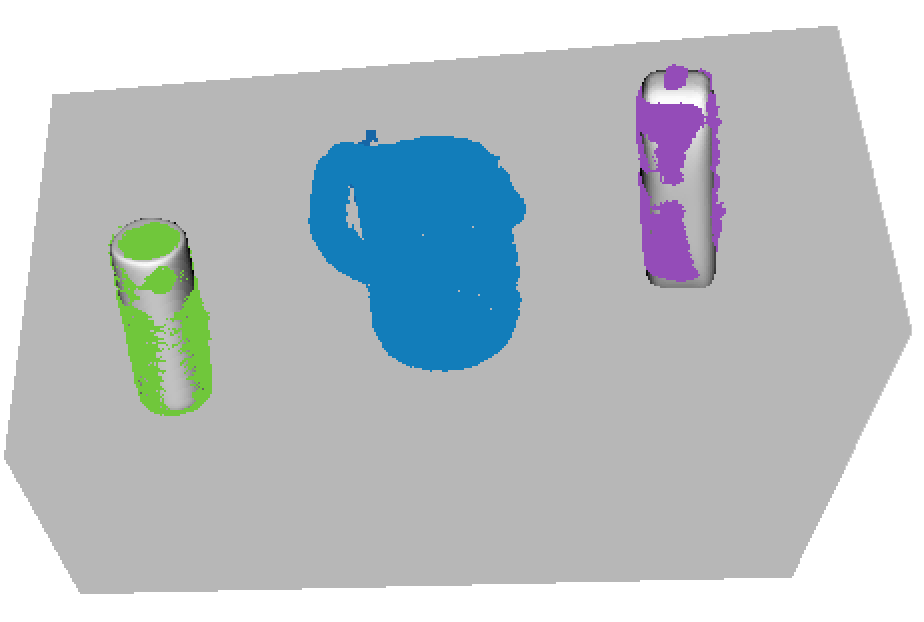
\includegraphics[width=0.45\columnwidth]{figures/rgbd_fitting_3}}
 \subfigure[]{
  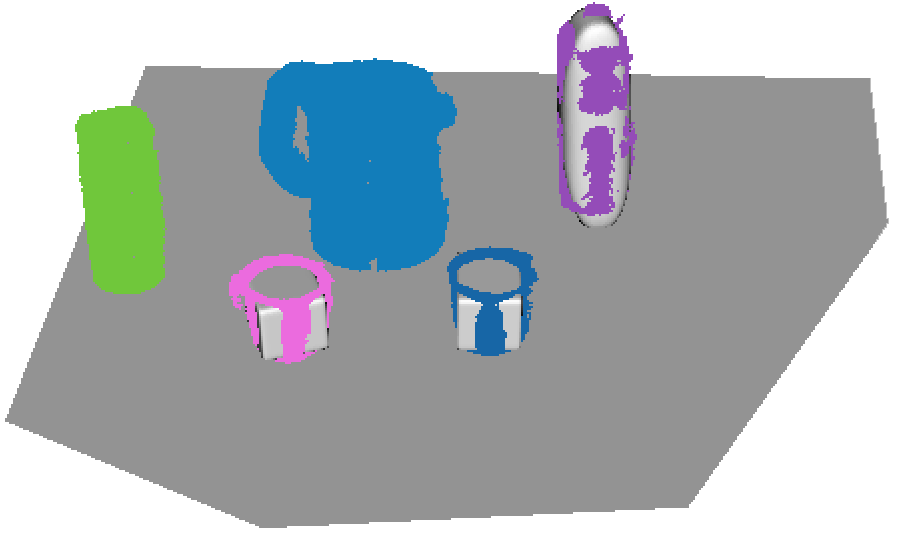
\includegraphics[width=0.45\columnwidth]{figures/rgbd_fitting_4}}
 \subfigure[]{
  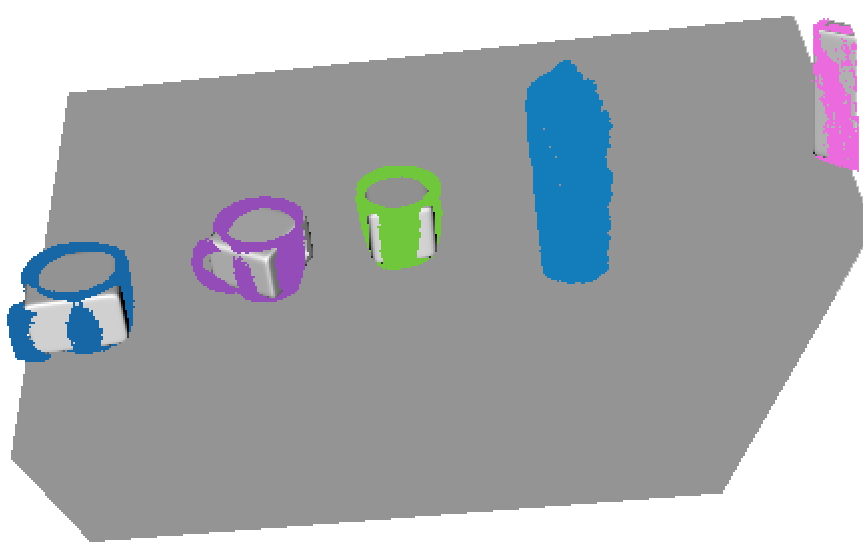
\includegraphics[width=0.45\columnwidth]{figures/rgbd_fitting_5}}

\caption{Superquadric fitting results of segmented RGB-D data}
\label{fig:rgbd_fitting}
\end{figure}


\begin{table}
\centering
\begin{tabular}{| c | c | c |}
\hline
Dataset & Segmentation time [s] & Successful cluster fitting [s] \\
\hline
kinfu\_1 & 22.3 & 6.2 \\
kinfu\_2 & 28.7 & 6.4 \\
kinfu\_3 & 20.8 & 5.8 \\
kinfu\_4 & 22.3 & 6.2 \\
kinfu\_5 & 28.4 & 5.5 \\
\hline
\end{tabular}

\caption {Performance timing of superquadric fitting on segmented RGB-D data.}
\label {table:rgbd_fitting_timing}
\end{table}


\subsection*{Superquadric detection in real RGB-D data}

Next, we look into the object detection pipeline and apply to our tabletop context. We perform superquadric object detection with the parameters learnt for a bottle for each cluster separately. The results are shown in Figure \ref{fig:rgbd_detection}.

\begin{figure}
\centering
 \subfigure[]{
  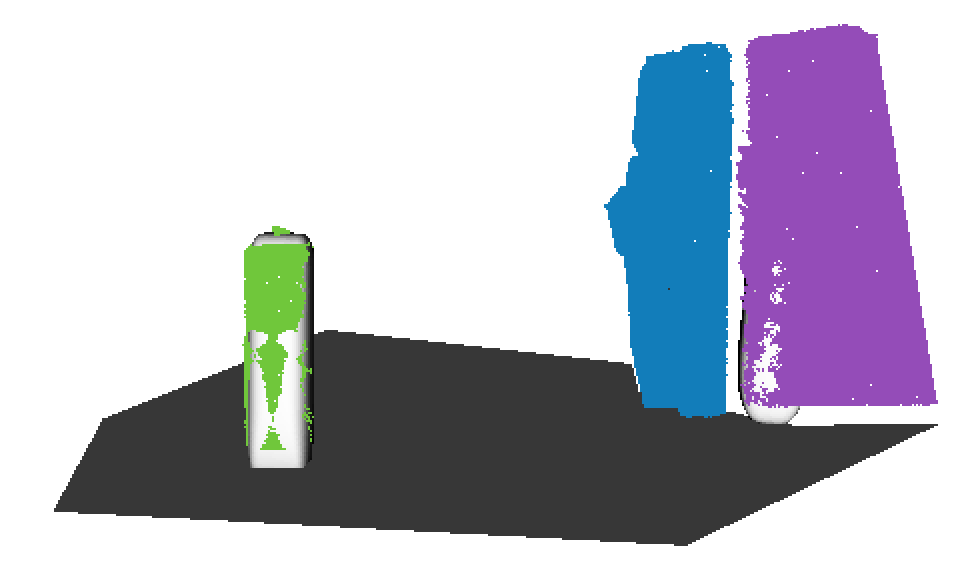
\includegraphics[width=0.45\columnwidth]{figures/rgbd_detection_1}}
 \subfigure[]{
  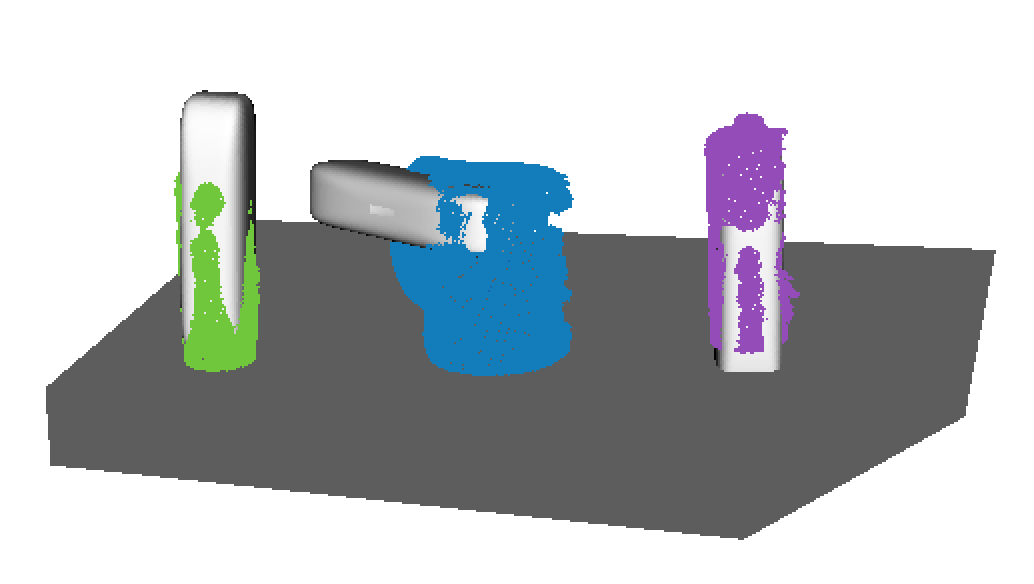
\includegraphics[width=0.45\columnwidth]{figures/rgbd_detection_2}}
 \subfigure[]{
  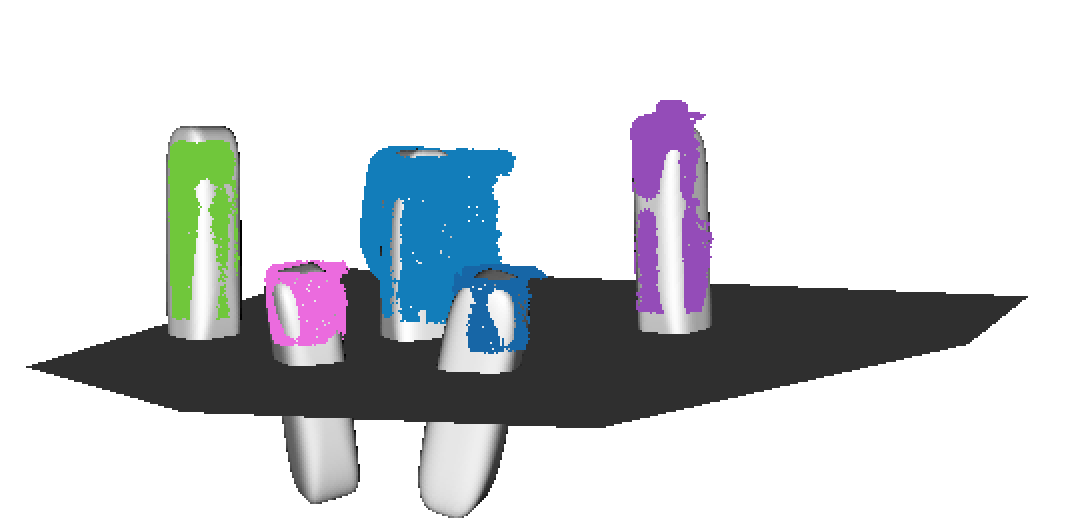
\includegraphics[width=0.45\columnwidth]{figures/rgbd_detection_3}}

\caption{Superquadric detection results of segmented RGB-D data}
\label{fig:rgbd_detection}
\end{figure}



\section {Conclusion and Future Work}
\label{sec:conclusion}

We have presented the theoretical background and the results we obtained during the second Toyota Code Sprint in collaboration with Open Perception. The outcome encourages to continue exploring the possible applications of parametric models in order to describe real world scans for robotics or commercial applications.

For future work, we will look into the following:

\begin{itemize}
	\item {integrate the code into PCL - this has been currently avoided due to the additional dependency to CERES and due to the highly experimental status of the implementations.}
	\item {tutorial/article on the PCL website to attract attention to the results of the project and get external feedback, or possible ideas for improvement.}
	\item {evaluate the superquadric fitting using a vfh\_clustering type algorithm and compare it to other state-of-the-art object detection/fitting approaches.}
	\item {explore further possibilities of point cloud data modeling, such as \cite{li_globFit_sigg11}, \cite{Shen:2012:SRP:2366145.2366199}}
	\item {superquadrics with global deformations.}
	\item {look into using different parametric solid models, other than superquadrics, that might yield more descriptive power.}
\end{itemize}


\newpage
\bibliography{references}
\bibliographystyle{plain}


\end{document}